\documentclass{article}
\usepackage[utf8]{inputenc}
\usepackage[spanish]{babel}
\usepackage{listings}
\usepackage{hyperref}
\usepackage{multirow}
\usepackage{graphicx}
\usepackage{amsmath}
\usepackage{graphicx}
\usepackage{fancyhdr}
\usepackage{geometry}
\usepackage{array}
\usepackage{float}
\usepackage{xcolor}
\usepackage{tcolorbox}
\geometry{a4paper, margin=1in}
\usepackage{booktabs} % Para líneas más bonitas en las tablas

%Aumentar el tamaño de fuente
\renewcommand{\normalsize}{\fontsize{12}{14}\selectfont}


% Información reutilizable
\newcommand{\myTitle}{Teoría del tema 2: Existencias: Compras y Ventas}
\newcommand{\myAuthor}{Ismael Sallami Moreno}
\newcommand{\myDegree}{Doble Grado Ingeniería Informática y Administración y Dirección de Empresas}
\newcommand{\mySubject}{Contabilidad Financiera I}
\newcommand{\myDate}{\today}

% cambiando la fuente

\begin{document}

% Portada
\begin{titlepage}
    \centering
    \begin{minipage}{0.45\textwidth}
        \centering
        
\includegraphics[width=0.8\textwidth]{../images/logo_ugr.jpg}
    \end{minipage}    \hfill
    \begin{minipage}{0.45\textwidth}
        \centering
        
\includegraphics[width=0.8\textwidth]{../images/logo_economicas.jpg} 
    \end{minipage}
    \vspace{1cm}
    
    {\scshape\LARGE \myDegree \par}
    \vspace{1cm}
    {\scshape\Large \mySubject \par}
    \vspace{1.5cm}
    {\huge\bfseries \myTitle \par}
    \vspace{2cm}
    {\Large\itshape \myAuthor \par}
    \vfill
    \myDate\par
\end{titlepage}

\tableofcontents
\newpage

\section{INTRODUCCIÓN}

El objetivo principal de esta unidad didáctica consiste, en primer lugar, en conocer que se entiende por existencias, analizar sus principales características y tipología. A continuación, se establecen cuáles son los criterios de valoración de entrada de estas existencias, así como los criterios de asignación de valor de las mismas con el fin de determinar el coste de las ventas y el valor de las existencias finales. Se realiza una primera toma de contacto con la Norma de valoración 14 del PGC sobre los ingresos por ventas y prestación de servicios, así como sobre la contabilización del impuesto de valor añadido. Por último, se analizan una serie de operaciones vinculadas a las existencias y se hace referencia a cómo se presenta en las Cuentas Anuales la información relativa a las mismas.

\section{EXISTENCIAS: CONCEPTO, CARACTERÍSTICAS Y TIPOLOGÍA}

El Plan General de Contabilidad (PGC) define las existencias en la misma línea que la Norma Internacional de Contabilidad 2 (Existencias), NIC 2.

\begin{itemize}
    \item Las existencias son activos poseídos para:
    \begin{itemize}
        \item Ser vendidos en el curso normal de las operaciones de explotación.
        \item Incorporarse al proceso de producción.
        \item Ser consumidos en el proceso de producción o en la prestación de servicios.
    \end{itemize}
    \item Así, se diferencian tres tipos de existencias según el destino de las mismas:
    \begin{itemize}
        \item Activos poseídos para su venta sin transformación.
        \item Activos poseídos para transformar.
        \item Activos poseídos para utilizar en cualquier fase del proceso de transformación de bienes y servicios.
    \end{itemize}
\end{itemize}


Los subgrupos y cuentas relativas a las existencias contempladas en el PGC son los que se detallan en la figura 1.

\begin{figure}[H]
    \centering
    \begin{tabular}{|p{4cm}|p{4cm}|p{4cm}|}
        \hline
        \textbf{Tipo de existencia} & \textbf{Subgrupo} & \textbf{Cuenta} \\
        \hline
        \multirow{3}{*}{\rotatebox{90}{\parbox{2cm}{Adquiridas del exterior}}} & 30. Comerciales & 300. Mercaderías \\
        \cline{2-3}
        & 31. Materias Primas & 310. Materias primas \\
        \cline{2-3}
        & \multirow{6}{*}{\parbox{2cm}{32. Otros aprovisionamientos}} & 320. Elementos y conjuntos incorporables \\
        \cline{3-3}
        & & 321. Combustible \\
        \cline{3-3}
        & & 322. Repuestos \\
        \cline{3-3}
        & & 325. Materiales Diversos \\
        \cline{3-3}
        & & 326. Embalajes \\
        \cline{3-3}
        & & 327. Envases \\
        \cline{3-3}
        & & 328. Material de Oficina \\
        \hline
        \multirow{5}{*}{\rotatebox{90}{\parbox{2cm}{Surgidas del proceso productivo}}} & 33. Productos en curso & 330. Productos en curso \\
        \cline{2-3}
        & 34. Productos semiterminados & 340. Productos semiterminados \\
        \cline{2-3}
        & 35. Productos terminados & 350. Productos terminados \\
        \cline{2-3}
        & 36. Subproductos, residuos y materiales recuperados & 360. Subproductos \\    \cline{3-3}
        & & 365. Residuos \\
        \cline{3-3}
        & & 368. Material recuperado \\
        \hline
    \end{tabular}
    \caption{Subgrupos y cuentas del PGC relacionadas con las existencias}
\end{figure}

El subgrupo 30 es propio de las empresas comerciales, es decir, las adquiridas del exterior que no requieren de un proceso de modificación física o fabricación en la empresa, y los subgrupos 31, 33, 34, 35, 36 y la cuenta 320 son propios de las empresas industriales, donde sí se produce un proceso de modificación de las materias inicialmente adquiridas e incluidas en un proceso de fabricación, mientras que el resto de los subgrupos pueden ser compartidos por cualquier empresa. A continuación, la figura 2 incluye las definiciones de los distintos subgrupos, según indica el PGC en su segunda parte:

\begin{figure}[h]
    \centering
    \begin{tabular}{|m{2cm}|m{3cm}|m{6cm}|}
        \hline
        \textbf{Subgrupo} & \textbf{Denominación} & \textbf{Definición} \\
        \hline
        30 & Comerciales & Bienes adquiridos por la empresa y destinados a la venta sin transformación. \\
        \hline
        31 & Materias primas & Las que, mediante elaboración o transformación, se destinan a formar parte de los productos fabricados. \\
        \hline
        32 & (320) Elementos y conjuntos incorporables & Los fabricados normalmente fuera de la empresa y adquiridos por ésta para incorporarlos a su producción sin someterlos a transformación. \\
        \hline
    \end{tabular}
    \caption{Tipología de existencias, subgrupo y definición}
\end{figure}

\section*{Existencias no sometidas a transformación}

\begin{tabular}{|p{4cm}|p{4cm}|p{6cm}|}
\hline
\textbf{Subgrupo} & \textbf{Denominación} & \textbf{Definición} \\
\hline
32 & (321) Combustibles & Materias energéticas susceptibles de almacenamiento. \\
\hline
32 & (322) Repuestos & Piezas destinadas a ser montadas en instalaciones, equipos o máquinas en sustitución de otras semejantes. Se incluirán en esta cuenta las que tengan un ciclo de almacenamiento inferior a un año. \\
\hline
32 & (325) Materiales diversos & Otras materias de consumo que no han de incorporarse al producto fabricado. \\
\hline
32 & (326) Embalajes & Cubiertas o envolturas, generalmente irrecuperables, destinadas a resguardar productos o mercaderías que han de transportarse. \\
\hline
32 & (327) Envases & Recipientes o vasijas, normalmente destinadas a la venta juntamente con el producto que contienen. \\
\hline
32 & (328) Material de oficina & El destinado a la finalidad que indica su denominación, salvo que la empresa opte por considerarlo que el material de oficina adquirido durante el ejercicio es objeto de consumo en el mismo. \\
\hline
\end{tabular}

\section*{Existencias sometidas a transformación}

\begin{tabular}{|p{4cm}|p{4cm}|p{4cm}|}
\hline
\textbf{Subgrupo} & \textbf{Denominación} & \textbf{Definición} \\
\hline
33 & Productos en curso & Bienes o servicios que se encuentran en fase de formación o transformación en un centro de actividad al cierre del ejercicio y que no deban registrarse en las cuentas de los subgrupos 34 o 36. \\
\hline
34 & Productos semiterminados & Los fabricados por la empresa y no destinados normalmente a su venta hasta tanto sean objeto de elaboración, incorporación o transformación posterior. \\
\hline
35 & Productos terminados & Los fabricados por la empresa y destinados al consumo final o a su utilización por otras empresas. \\
\hline
36 & (360) Subproductos & Los de carácter secundario o accesorio de la fabricación principal. \\
\hline
36 & (365) Residuos & Los obtenidos inevitablemente y al mismo tiempo que los productos o subproductos, siempre que tengan valor intrínseco y puedan ser utilizados o vendidos. \\
\hline
36 & (368) Materiales recuperables & Los que, por tener valor intrínseco, entran nuevamente en almacén después de haber sido utilizados en el proceso productivo. \\
\hline
\end{tabular}

\section*{}

Un caso que requiere una mención especial, y que se recoge en el epígrafe 2.4.8 del presente capítulo, es la incorporación del concepto de prestación de servicios en las existencias, registrándolos al coste de producción siempre que no se hayan reconocido los ingresos correspondientes a los mismos.

\section{Reconocimiento y Valoración Inicial de las Existencias}

Uno de los aspectos más importantes de las existencias se refiere a su valoración por el efecto que esto ocasiona en la situación patrimonial y en la cuenta de resultados de la empresa. En este sentido, resulta necesario, en primer lugar, establecer un marco general de valoración de estas existencias, donde se establezcan, principalmente, las diferencias en cuanto a su forma de adquisición, así como, el criterio de valoración de las entradas, y el método de asignación de valor de las salidas, el cual se encuentra recogido en la figura 3.

\begin{figure}[H]
    \centering
    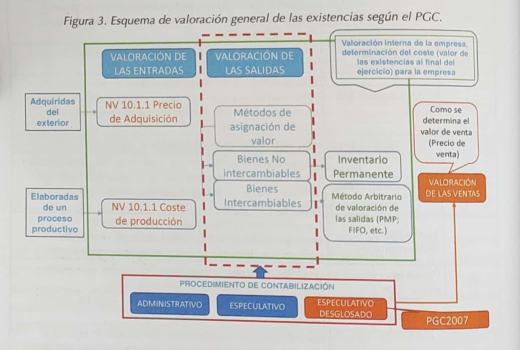
\includegraphics[width=\textwidth]{figura3.png}
    \caption{Esquema de valoración general de las existencias según el PGC.}
\end{figure}

\subsection{Valoración de las Entradas}
\begin{itemize}
    \item Adquiridas del exterior
    \begin{itemize}
        \item NV 10.1.1 Precio de Adquisición
    \end{itemize}
    \item Elaboradas de un proceso productivo
    \begin{itemize}
        \item NV 10.1.1 Coste de producción
    \end{itemize}
\end{itemize}

\subsection{Valoración de las Salidas}
\begin{itemize}
    \item Métodos de asignación de valor
    \begin{itemize}
        \item Bienes No Intercambiables
        \item Bienes Intercambiables
    \end{itemize}
    \item Inventario Permanente
    \begin{itemize}
        \item Método Arbitrario de valoración de las salidas (PMP, FIFO, etc.)
    \end{itemize}
\end{itemize}

\subsection{Valoración de las Ventas}
\begin{itemize}
    \item Valoración Interna de la empresa, determinación del coste (valor de las existencias al final del ejercicio) para la empresa
    \item Cómo se determina el valor de venta (Precio de venta)
\end{itemize}

\subsection{Procedimiento de Contabilización}
\begin{itemize}
    \item Administrativo
    \item Especulativo
    \item Especulativo Desglosado
\end{itemize}

\subsection{Valoración de las entradas de existencias}

Partiendo del esquema presentado en la figura 3, la NV 10 señala que los bienes y servicios comprendidos en las existencias se valorarán por su coste, ya sea el precio de adquisición o el coste de producción, ya sean adquiridos en el exterior o producidos por la empresa, respectivamente.

\subsubsection{Precio de adquisición de las existencias}

Concretamente, el precio de adquisición está formado por el importe facturado por el proveedor más todos los gastos adicionales que se produzcan hasta que los bienes se encuentren ubicados para su venta, tales como transportes, aranceles de aduanas, seguros y otros directamente atribuibles a la adquisición de existencias.

Los impuestos indirectos que gravan las existencias solo se incluirán en el precio de adquisición o coste de producción cuando no sean recuperables directamente de la Hacienda Pública (NV10 PGC).

En concreto, los gastos adicionales son:
\begin{itemize}
    \item Transportes, fletes y comisiones con cargo al comprador.
    \item Seguro, depósito y custodia en tránsito.
    \item Impuestos satisfechos por la compra no recuperables, incluidos aranceles y otros derechos.
    \item Inspección y conservación, si son por cuenta del comprador.
\end{itemize}

En las existencias que necesiten un periodo de tiempo superior a un año para estar en condiciones de ser vendidas, se incluirán en el precio de adquisición o coste de producción, los gastos financieros, en la medida en que se devenguen hasta el momento de inmovilizado material.

Del importe facturado por el proveedor se deducirá cualquier descuento, rebaja o bonificación y otras partidas similares, como los intereses incorporados al nominal de las deudas por adquisición en condiciones de aplazamiento, incluidos los no comerciales o financieros.

A modo de esquema, la valoración inicial incluiría:

\textbf{Figura 4. Esquema de valoración general de las existencias según el PGC}

\begin{itemize}
    \item PRECIO DE COMPRA/FACTURA
    \begin{itemize}
        \item Importe facturado
        \item (-) Descuentos y rebajas
    \end{itemize}
    \item (+) Impuestos no recuperables (NV.10.1) no recuperables:
    \begin{itemize}
        \item Gastos financieros (si se devengan hasta el momento de inmovilizado material NV.10.1)
        \item Seguros, depósitos y custodia en tránsito
        \item Inspección y conservación
    \end{itemize}
    \item (+) OTROS GASTOS ADICIONALES:
    \begin{itemize}
        \item Transporte
        \item Aranceles y otros impuestos no recuperables directamente de la Hacienda Pública
        \item Comisiones con cargo al comprador
        \item Otros gastos directamente atribuibles hasta que los bienes se hallen ubicados para su venta
    \end{itemize}
\end{itemize}

\section*{Ejemplo 1}

Una empresa adquiere 800 unidades de una mercancía a un precio unitario de 75 €. Además, se obtiene un descuento comercial de 2.000 € y un descuento por pronto pago fuera de factura de 200 €. Los aranceles de la aduana ascienden a 600 €. La empresa incurre en unos gastos de transporte de la mercancía hasta su almacén por importe de 5.000 € y de seguro por importe de 2.000 €. El proveedor concede un descuento de 500 € en el caso de que se superen las 3.000 unidades de compra al año. Los costes de administración y almacenamiento de las mercancías ascienden a 1.600 €.

\section*{Solución}

Veamos el proceso de cálculo del precio de adquisición en base a la normativa contable anteriormente.

\begin{align*}
\text{Importe de la adquisición (800 unidades al precio de 75 €)} &= 60.000 € \\
\text{- Descuento comercial} &= -2.000 € \\
\text{+ Aranceles} &= +600 € \\
\text{+ Gastos de transporte} &= +5.000 € \\
\text{+ Seguros} &= +2.000 € \\
\text{Precio de Adquisición} &= 65.600 €
\end{align*}

\subsubsection{Coste de producción de las existencias}

El coste de producción de las existencias en una empresa industrial se determina sumando al precio de adquisición de las materias primas y otras materias consumibles, los costes directamente imputables al producto. También se incluyen los costes indirectos atribuibles al producto.

El coste de estos productos se valora aplicando el criterio del coste de producción, que se usa para valorar las existencias de productos terminados, productos semiterminados, y productos en curso.

Los elementos que forman el coste de producción son los siguientes:

\begin{itemize}
    \item \textbf{Costes directos:} Incluyen el precio de adquisición de la materia prima y otras materias consumibles, así como los costes directamente imputables al producto, como la mano de obra directa.
    \item \textbf{Costes indirectos:} Son aquellos que no se pueden identificar directamente en los productos y requieren criterios de reparto para determinar la parte correspondiente a cada producto. Ejemplos de estos costes son los derivados de la utilización de la capacidad normal de trabajo de los medios de producción.
\end{itemize}

Es importante considerar también los anticipos a proveedores, que afectan al concepto de existencias en la cuenta de suministros futuros de existencias y se valorarán al coste. Los débitos por operaciones comerciales se valorarán de acuerdo con la norma relativa a instrumentos financieros.

\subsection{Métodos de asignación de valor}

De acuerdo con la NV. 10.1.3, se pueden utilizar diferentes métodos de asignación de valor de las existencias según sean intercambiables o no. Los bienes no intercambiables son aquellos que son fácilmente distinguibles del resto. Cuando una empresa produce o comercializa bienes no intercambiables, se asigna valor identificando el precio o costos específicos de cada bien individualmente.

Para bienes intercambiables, se usa generalmente el método del precio medio o coste medio ponderado. El método FIFO es aceptable si es más conveniente para la gestión de la empresa. Es importante que se mantenga un único método de asignación de valor para todas las existencias con naturaleza y uso similares, siguiendo el principio de uniformidad del PGC.

\subsubsection{Precio Medio Ponderado o Coste Medio Ponderado}
Este criterio consiste en la realización de una valoración homogénea de todos los artículos del almacén. El valor de coste de la venta es la media ponderada de los distintos precios de entrada en función del volumen de unidades adquiridas a cada uno de los precios, tal y como puede apreciarse en la siguiente fórmula.

\begin{equation}
\text{Cálculo del Precio o Coste Medio Ponderado} = \frac{(q_1 \times p_1) + (q_2 \times p_2) + \ldots + (q_n \times p_n)}{q_1 + q_2 + \ldots + q_n}
\end{equation}

Donde, $q$ es la cantidad de producto adquirido, y $p$ es el precio al que fue adquirido el producto $n$.

\subsubsection{FIFO (First in first out, Primera Entrada - Primera salida)}
El coste de la venta será el más antiguo de los precios de adquisición existentes, y las existencias finales coincidirán con las últimas entradas en el almacén de mercancías.

Veamos el siguiente ejemplo de valoración de las salidas, utilizando la ficha de inventario.

\section*{Ejemplo 2.2}

Una empresa comercial presenta los siguientes movimientos de almacén del producto X para el mes de enero del ejercicio económico 2020.

\begin{table}[h]
\centering
\caption{Movimientos de almacén del producto X}
\begin{tabular}{llll}
\toprule
Concepto & Fecha & Unidades & Precio unitario \\
\midrule
Existencia inicial & 1 de enero & 300 & 2 \\
Compra & 10 de enero & 500 & 2.5 \\
Venta & 15 de enero & 400 &  7 \\
Compra & 20 de enero & 400 & 3 \\
Venta & 25 de enero & 600 & 15 \\
\bottomrule
\end{tabular}
\end{table}

\textbf{SE PIDE:} Determinar el coste de las ventas y realizar la valoración de las existencias finales, aplicando el criterio PMP y FIFO.

\subsection*{Solución}

En primer lugar, planteamos la solución del ejercicio siguiendo el criterio del PMP.

\subsubsection*{Criterio PMP}

Como se ha comentado en la exposición teórica, el PMP busca obtener un precio medio ponderado para hacer la valoración del coste de las salidas. En este sentido, conforme se van añadiendo diferentes existencias con diferentes costes, es necesario calcular este nuevo precio ponderado. En la tabla siguiente, el primer cálculo del PMP se produce cuando se realiza la primera compra del 10 de enero.

En ese momento tenemos dos precios distintos, el precio de compra de esta misma fecha y el precio de las existencias iniciales, por lo que hay que calcular el precio medio ponderado. La siguiente fecha donde hay que volver a calcular este nuevo precio es el 20 de enero, en ese momento, se produce la adquisición de un nueva tipo de existencia a otro precio distinto. La adquisición de nuevas compras de existencias con precios distintos cambia el precio medio ponderado, tal y como puede apreciarse en la columna existencias, en las fechas a las que hemos hecho referencia.

\section*{Ejemplo 2}

Una empresa comercial presenta los siguientes movimientos de almacén del producto X para el mes de enero del ejercicio económico 2020:

\begin{tabular}{|c|c|c|c|}
\hline
\textbf{Concepto} & \textbf{Fecha} & \textbf{Unidades} & \textbf{Precio unitario} \\
\hline
Existencia inicial & 1 de enero & 300 & 2 \\
\hline
Compra & 10 enero & 500 & 2,5 \\
\hline
Venta & 15 enero & 400 & 7 \\
\hline
Compra & 20 enero & 400 & 3 \\
\hline
Venta & 25 enero & 600 & 15 \\
\hline
\end{tabular}

\subsection*{SE PIDE}
Determinar el coste de las ventas y realizar la valoración de las existencias finales, aplicando el criterio PMP y FIFO.

\subsection*{PMP}
\textbf{Solución}

En primer lugar, planteamos la solución del ejercicio siguiendo el criterio del Precio Medio Ponderado (PMP).

\section*{Criterio PMP}

Como se ha comentado en la exposición teórica, el PMP busca obtener un precio medio ponderado para hacer la valoración del coste de las salidas. Conforme se van añadiendo diferentes existencias con diferentes costes es necesario calcular este nuevo precio ponderado. En la tabla siguiente, el primer cálculo del PMP se produce cuando se realiza la primera compra del 10 de enero. En ese momento tenemos dos precios distintos: el precio de compra de esta misma fecha y el precio de las existencias iniciales, por lo que hay que calcular el precio medio ponderado. La siguiente fecha donde hay que volver a calcular este nuevo precio es el 20 de enero, cuando se produce la adquisición de un nuevo tipo de existencia a otro precio distinto. La adquisición de nuevas compras de existencias con precios distintos cambia el precio medio ponderado, tal y como puede apreciarse en la columna existencias, en las fechas a las que hemos hecho referencia.

\begin{table}[H]
    \centering
    \begin{tabular}{|c|ccc|ccc|ccc|}
    \hline
    \textbf{FECHA} & \multicolumn{3}{c|}{\textbf{ENTRADAS}} & \multicolumn{3}{c|}{\textbf{SALIDAS}} & \multicolumn{3}{c|}{\textbf{EXISTENCIAS}} \\
    \hline
     & \textbf{U} & \textbf{P} & \textbf{CT} & \textbf{U} & \textbf{P} & \textbf{CT} & \textbf{U} & \textbf{P} & \textbf{CT} \\
    \hline
    1/1 & 300 & 2 & 600 &  &  &  & 300 & 2 & 600 \\
    \hline
    10/1 & 500 & 2.5 & 1,250 &  &  &  & 300 &  &  \\
     &  &  &  &  &  &  & 500 & 2.3125 & 1,850 \\
     &  &  &  &  &  &  & 800 &  &  \\
    \hline
    15/1 &  &  &  & 400 & 2.3125 & 925 & 400 & 2.3125 & 925 \\
     &  &  &  &  &  &  & 400 &  &  \\
     &  &  &  &  &  &  & 800 &  &  \\
    \hline
    20/1 & 400 & 3 & 1,200 &  &  &  & 400 & 2.65625 & 2,125 \\
     &  &  &  &  &  &  & 400 &  &  \\
     &  &  &  &  &  &  & 800 &  &  \\
    \hline
    25/1 &  &  &  & 600 & 2.65625 & 1,594 & 200 & 2.65625 & 531 \\
    \hline
    \textbf{TOTAL} & 3,050 & 1,000 &  & 2,519 &  &  & 531 &  &  \\
    \hline
    \end{tabular}
\end{table}
    
    
    
Donde U son unidades, P es el precio y CT es el coste total.

\[
\text{PMP (10/1)} = \frac{600 + 1,250}{800} = 2.3125\]
\[\text{PMP (20/1)} = \frac{925 + 1,200}{800} = 2.65625
\]

\[
\text{Existencias finales (200 unidades)} = 531 \, \text{€}
\]
\[
\text{Coste de las ventas (1,000 unidades)} = 2,519 \, \text{€} \, (925 + 1,594)
\]

Cuando se producen las ventas en este supuesto, el 15 de enero y el 25 de enero, la empresa sabe que el coste de las mismas es de 2.31 € y de 2.65 €, respectivamente. Esto se traduce en que si la empresa quiere tener un beneficio contable siguiendo este criterio, el precio de venta por unidad debe ser superior a estos importes.

\section*{Solución Aplicando FIFO}

\section*{Criterio FIFO}

\textbf{Veamos a continuación cual sería la solución si aplicamos el criterio FIFO.}
\begin{table}[H]
    \centering
    \begin{tabular}{|c|ccc|ccc|ccc|}
    \hline
    \textbf{FECHA} & \multicolumn{3}{c|}{\textbf{ENTRADAS}} & \multicolumn{3}{c|}{\textbf{SALIDAS}} & \multicolumn{3}{c|}{\textbf{EXISTENCIAS}} \\
    \hline
     & \textbf{U} & \textbf{P} & \textbf{CT} & \textbf{U} & \textbf{P} & \textbf{CT} & \textbf{U} & \textbf{P} & \textbf{CT} \\
    \hline
    1/1 & 300 & 2 & 600 &  &  &  & 300 & 2 & 600 \\
    \hline
    10/1 & 500 & 2.5 & 1,250 &  &  &  & 300 & 2 & 600 \\
     &  &  &  &  &  &  & 500 & 2.5 & 1,250 \\
     &  &  &  &  &  &  & 800 &  & 1850 \\
    \hline
    15/1 &  &  &  & 300 & 2 & 600 &  &  &  \\
     &  &  &  & 100 & 2.5 & 250 & 400 & 2.5 & 1000  \\
     &  &  &  & 400 &  & 850 &  &  &  \\
    \hline
    20/1 & 400 & 3 & 1,200 &  &  &  & 400 & 2.5 & 1000 \\
     &  &  &  &  &  &  & 400 & 3 & 1200 \\
     &  &  &  &  &  &  & 800 &  & 2250  \\
    \hline
    25/1 &  &  &  & 400 & 2.5 & 1000 &  &  &  \\
    &  &  &  & 200  & 3 & 600 & 200 & 3 & 600 \\
    &  &  &  & 600 &  & 1600 &  &  &   \\    \hline
    \textbf{TOTAL} &  & & 3050 & 1000 &  & 2450 &  &  & 600 \\
    \hline
    \end{tabular}
    \caption{\textbf{CUIDADO}: en la columna de precios, estan en medio, los he puesto asi por facilidades.}
\end{table}

Para el caso de que la empresa utilice el criterio FIFO, ahora no se debe calcular ningún precio medio entre las existencias. En su lugar, las existencias se ordenan en función de su llegada. Para el caso que nos ocupa, la valoración que se le da a las salidas de las existencias es, en primer lugar, el precio que tienen las existencias iniciales. Posteriormente, se valoran las salidas por el precio de adquisición de las compras del 10 de enero y del 20 de enero, por ese orden.

No obstante, resulta conveniente analizar cómo afectan diferentes acciones que pueden llevarse a cabo y que pueden afectar a las existencias, determinando además su impacto en su coste y en el número de unidades de su inventario. A modo de resumen de la NV 10.2, las figuras 6 y 7 recogen estas acciones y su impacto.


\begin{table}[H]
    \centering
    \begin{tabular}{|p{3cm}|p{3cm}|p{3cm}|p{3cm}|}
    \hline
    \textbf{Concepto} & \textbf{¿Afecta a la valoración de existencias?} & \textbf{Coste unitario} & \textbf{Nº Unidades} \\
    \hline
    Compra & Sí & Sí & Sí \\
    \hline
    Venta & No & No & No \\
    \hline
    Descuentos s/compras por p.p. & Sí & Sí (disminuye) & Sí (disminuye) \\
    \hline
    Transportes s/compras & Sí & Sí (aumenta) & No \\
    \hline
    Transportes s/ventas & No & No & No \\
    \hline
    Descuento comercial compras & Sí & Sí (disminuye) & No \\
    \hline
    Descuento comercial ventas & No & No & No \\
    \hline
    Devolución de compras & Sí & Sí & No \\
    \hline
    Devolución de ventas & No & No & Sí (disminuye) \\
    \hline
    Rappels por compras & Sí (depende) & Sí (disminuye) & No \\
    \hline
    \end{tabular}
    \caption{Acciones relacionadas con las existencias e impacto sobre su valoración (I) - NRV 10.2}
    \end{table}
    
    \begin{table}[H]
    \centering
    \begin{tabular}{|p{3cm}|p{3cm}|p{3cm}|p{3cm}|}
    \hline
    \textbf{Concepto} & \textbf{¿Afecta a la valoración de existencias?} & \textbf{Coste unitario} & \textbf{Nº Unidades} \\
    \hline
    Rappels sobre ventas & No & No & No \\
    \hline
    Aranceles e impuestos no repercutibles sobre compras & Sí & Sí (aumenta) & No \\
    \hline
    Subvenciones y compensaciones de compras & Sí & Sí (disminuye) & No \\
    \hline
    Otros gastos sobre compras & Sí & Sí (aumenta) & No \\
    \hline
    Gastos de venta & No & No & No \\
    \hline
    \end{tabular}
    \caption{Acciones relacionadas con las existencias e impacto sobre su valoración (II) - NRV 10.2}
    \end{table}

    \section{Valoración posterior de las existencias}


Una vez registradas las existencias según su valoración inicial, es necesario realizar una valoración posterior para establecer su valor final en las cuentas anuales al final del ejercicio. Esta nueva valoración implica ajustar el valor mediante correcciones que, en el mejor de los casos, mantendrán la valoración inicial, sin poder superarla. Estos ajustes se denominan correcciones valorativas.

Es importante diferenciar entre el deterioro de valor, que es una pérdida reversible, y la pérdida de valor definitiva, que es irreversible. Por ejemplo, el deterioro puede revertirse si se recupera el valor original, mientras que una pérdida por causas como una inundación es definitiva.
\begin{figure}[H]
    \centering
    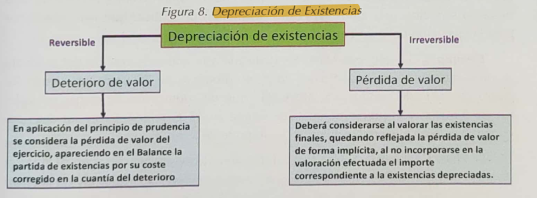
\includegraphics[width=\textwidth]{figura4.png}
\end{figure}

Cuando el valor neto realizable de las existencias es inferior al precio de adquisición o coste de producción, se deben hacer correcciones valorativas y reconocerlas como un gasto en la cuenta de pérdidas y ganancias. Si las causas de la corrección desaparecen, la corrección se revierte y se reconoce como ingreso.

El valor realizable de un activo es el importe que se puede obtener por su venta en el mercado, deduciendo los costes necesarios para la transacción y para terminar la producción si aplica.

No se realizará corrección valorativa en materias primas si los productos terminados se venderán por encima del coste. Si se requiere corrección, el precio de reposición puede ser la mejor medida. Bienes o servicios sujetos a contratos de venta no se corrigen si el precio cubre al menos el coste de las materias primas y otros costes necesarios.

\section*{Ejemplo 3}

La empresa ALFA, SA dedicada a la comercialización del producto X, presenta unas existencias finales de dicho producto de 75 unidades, siendo los gastos de venta del producto 1.500 €. El coste de adquisición de dichas unidades fue de 3.500 € y el precio de venta se estima en 47 €/unidad. Existe un deterioro contabilizado en el ejercicio anterior por importe de 5.000 €.

\textbf{SE PIDE:} Contabilizar, si procede, el deterioro de existencias.

\begin{table}[H]
    \centering
    \begin{tabular}{|l|r|}
        \hline
        \textbf{Concepto} & \textbf{Importe} \\
        \hline
        Coste de adquisición & 3.500 € \\
        \hline
        Valor neto realizable (75 x 47) - 1.500 & 2.025 € \\
        \hline
        Deterioro & 1.475 € \\
        \hline
    \end{tabular}
\end{table}

\begin{table}[H]
    \centering
    \begin{tabular}{|p{4cm}|p{4cm}|p{4cm}|}
        \hline
        \textbf{DEBE} & \textbf{Por la corrección valorativa, al cierre del ejercicio} & \textbf{HABER} \\
        \hline
        1.475 & (693) Pérdidas por deterioro de existencias &  \\
         & (390) Deterioro de valor de las mercaderías & 1.475 \\
        \hline
    \end{tabular}
\end{table}

Tal y como se ha comentado en la exposición teórica, una vez dotada la corrección valorativa del año en curso, procede, en el caso de que existiera, la anulación del deterioro del ejercicio anterior, tal y como se refleja en el siguiente asiento contable.

\begin{table}[H]
    \centering
    \begin{tabular}{|p{4cm}|p{4cm}|p{4cm}|}
        \hline
        \textbf{DEBE} & \textbf{Por la anulación, al cierre, del deterioro del ejercicio anterior} & \textbf{HABER} \\
        \hline
        5.000 & (390) Deterioro de valor de las mercaderías &  \\
         & (793) Reversión del deterioro de existencias & 5.000 \\
        \hline
    \end{tabular}
\end{table}

\section*{Ejemplo 4.-} A 30 de noviembre de 2019 la compañía ZZ, dedicada a la comercialización de consumibles informáticos, poseía en su almacén 11.000 dispositivos valorados en 104.500 €. Sin embargo, el recuento de existencias realizado a 31/12/2019 descubre que 1.000 dispositivos han sido robados, por lo que las existencias finales ascienden a 10.000 dispositivos valorados en 95.000 €. Según un estudio de mercado realizado, estos 10.000 dispositivos podrían venderse por 100.000 €, para lo que habría que atender gastos de comercialización (comisiones de venta) por importe de 10.000 €.

Además, a 31 de diciembre de 2020 los datos relativos a las existencias en almacén son los siguientes:
\begin{itemize}
    \item Nº de dispositivos: 14.000
    \item Precio unitario de coste: 10 €
    \item Valor de mercado: 150.000 €
    \item Gastos de comercialización: 8.000 €
\end{itemize}

\textbf{SE PIDE:} Contabilizar, si procede, el deterioro de existencias.

\textbf{Solución:}

En primer lugar, tenemos que considerar cómo afectan al registro contable los 1.000 dispositivos robados. Téngase en cuenta que esos dispositivos se contabilizaron cuando se produjo su adquisición mediante un asiento contable de compras de mercaderías. En este sentido, cabe plantearse qué acción contable es requerida cuando se pone de manifiesto la existencia de un robo. En este caso, no procede realizar un asiento contable que refleje esta pérdida, porque realmente no se ha producido ninguna salida, el ajuste debe realizarse en la valoración que la empresa hace de sus existencias, es decir, en la ficha de inventario, por lo que la pérdida queda recogida en el momento de realizar el asiento de variación de existencias.

\section*{Corrección de valor por deterioro de existencias}

\begin{table}[H]
    \centering
    \begin{tabular}{|p{4cm}|p{4cm}|p{4cm}|}
        \hline
        \textbf{DEBE} & \textbf{Baja en inventario de los 1.000 dispositivos robados} & \textbf{HABER} \\
        \hline
        & No procede asiento. La baja ya está incorporada en el valor de las existencias finales. & \\
        \hline
    \end{tabular}
\end{table}

Por tanto, la empresa tiene unas existencias finales de 95.000 €, pero hay que tener en cuenta la posible existencia de un deterioro de valor al proporcionar el enunciado información sobre la existencia de un valor de mercado. Teniendo en cuenta este valor y los gastos de comercialización es posible determinar el valor realizable neto de las mismas.

\begin{table}[H]
\centering
\begin{tabular}{|l|l|l|}
\hline
\textbf{DEBE} & \textbf{Posible corrección valorativa a 31/12/2019} & \textbf{HABER} \\
\hline
5.000 & (693) Pérdidas por deterioro de existencias & \\
 & (390) Deterioro de valor de las mercaderías & 5.000 \\
\hline
\end{tabular}
\end{table}

Valor realizable neto (VRN\(_{2019}\)) = 100.000 - 10.000 = 90.000 €; \\
¿Existe deterioro? Para ello comparamos VC y VRN; \\
El valor contable (VC) a finales de 2019 es 90.000 €, al ser este inferior al VRN\(_{2019}\) el cual asciende a 95.000 € (95.000 - 90.000 = 5.000), debemos dotar deterioro. \\

Cerrado el ejercicio de 2019, el siguiente proceso contable a estudiar es el final del ejercicio de 2020. En este caso, de nuevo se nos proporciona información relativa a un valor de mercado junto con unos gastos de comercialización, por lo que corresponde de nuevo analizar si existe la posibilidad de dotar deterioro.

\begin{table}[H]
    \centering
    \begin{tabular}{|l|l|l|}
    \hline
    \textbf{DEBE} & \textbf{Posible corrección valorativa a 31/12/2020} & \textbf{HABER} \\
    \hline
    5.000 & (693) Pérdidas por deterioro de existencias & \\
     & (793) Reversión del deterioro de las existencias & 5.000 \\
    \hline
    \end{tabular}
\end{table}
    
Valor realizable neto (VRN\(_{2020}\)) = 150.000 - 8.000 = 142.000 €; \\
¿Existe deterioro? Para ello comparamos VC y VRN; \\
El valor contable (VC) a finales de 2020 es 140.000 €, al ser este inferior al VRN\(_{2020}\) el cual asciende a 142.000 € no debemos dotar deterioro.\\

Tal y como ha quedado demostrado, no debemos dotar deterioro. No obstante, tal y como hemos comentado anteriormente, se debe proceder a anular el deterioro dotado en el ejercicio de 2019.

\section*{Ejemplo 5.-} La empresa EL TRAPO, S.L. dedicada a la comercialización de ropa, al 31 de diciembre de 2012 tiene en almacén ropa de verano por valor de 36.000 €, cuyo valor de mercado como fin de temporada es de 12.000 € (6). El día 1 de enero ha recibido una oferta de un cliente interesado en su adquisición para venderlo en Estados Unidos por 37.500 \$, con la condición de que la empresa EL TRAPO, S.L. se haga cargo del alquiler del local necesario para su distribución por importe total de 5.000 \$. (Cotización 1 \text{€} = 1 \$).

\textbf{SE PIDE:} Contabilizar, si procede, el deterioro de existencias planteando que TRAPO puede o no aceptar la condición del cliente americano.

\textbf{Solución:} Al considerarse como contrato de venta en firme, se aplica la norma de valoración 10ª. 2, en la que tenemos que comprobar si el precio de venta es superior a los costes, incluidos los pendientes de realizar del contrato:

\begin{itemize}
    \item (+) Precio de adquisición: 36.000
    \item (+) Costes pendientes de realizar que sean necesarios para la venta: 5.000
    \item (=) Total: 41.000
    \item (-) Precio venta estipulado: 37.500
    \item (=) Deterioro de valor: 3.500
    \item Valor de mercado de las existencias: 12.000

\end{itemize}


Si no acepta la oferta no estamos ante un contrato en firme y las existencias se valorarán al valor neto realizable a final del ejercicio.

\begin{table}[H]
\centering
\begin{tabular}{|p{4cm}|p{4cm}|p{4cm}|}
\hline
\textbf{a) Deterioro de valor, si procede, en el caso de no aceptar la propuesta del cliente} & \textbf{DEBE} & \textbf{HABER} \\
\hline
24.000 & (693) Pérdida por deterioro de valor de existencias. & \\
 & (390) Deterioro valor de las mercaderías & 24.000 \\
\hline
\end{tabular}
\end{table}

Precio de Adquisición - Valor neto realizable = 36.000 € - 12.000 €\\

Si acepta la oferta estamos ante un contrato de venta en firme y en este caso, debemos aplicar el criterio que establece la NV 10.2.

\begin{table}[H]
\centering
\begin{tabular}{|p{4cm}|p{4cm}|p{4cm}|}
\hline
\textbf{a) Deterioro de valor, si procede, en el caso de aceptar la propuesta del cliente} & \textbf{DEBE} & \textbf{HABER} \\
\hline
3.500 & (693) Pérdida por deterioro de valor de existencias. & \\
 & (390) Deterioro valor de las mercaderías & 3.500 \\
\hline
\end{tabular}
\end{table}

Precio de venta estipulado – costes 37.500 – (36.000 – 5.000) = -3.500; Los costes superan al precio de venta por lo que hay que dotar deterioro.

%2.4

\section{Procedimiento de contabilización de las existencias}


Otro aspecto importante es cómo se contabilizan las existencias. La cuenta de mercaderías puede seguir un procedimiento administrativo o especulativo. En el procedimiento administrativo, las entradas y salidas se registran a precio de coste en la cuenta de Existencias, ofreciendo un inventario contable permanente.

El procedimiento especulativo registra las ventas a precios de venta, incluyendo ganancias o pérdidas. El PGC utiliza el procedimiento especulativo desglosado, donde las operaciones con existencias se registran en cuentas diferentes a las de existencias, como compras y ventas. Las cuentas de existencias solo captan las existencias iniciales y finales, reflejando la variación de existencias.

En el caso de una empresa comercial se utilizan las siguientes cuentas:

\begin{itemize}
    \item \textbf{300} Mercaderías
    \item \textbf{600} Compras de mercaderías
    \item \textbf{606} Descuentos sobre compras por pronto pago
    \item \textbf{608} Devoluciones de compras y operaciones similares
    \item \textbf{609} Rappels por compras
    \item \textbf{610} Variación de existencias de mercaderías
    \item \textbf{700} Ventas de mercaderías
    \item \textbf{706} Descuentos sobre ventas por pronto pago
    \item \textbf{708} Devoluciones de ventas y operaciones similares
    \item \textbf{709} Rappels sobre ventas
\end{itemize}

\section*{Figura 9. Operativa de las cuentas relacionadas con la contabilización del procedimiento especulativo desglosado (I) - NV 10.2}

\begin{table}[H]
\centering
\begin{tabular}{|p{4cm}|p{4cm}|p{4cm}|p{4cm}|}
\hline
\textbf{Concepto de la transacción} & \textbf{Cuenta de registro} & \textbf{Cargo/Abono} & \textbf{Saldo D/H} \\
\hline
Adquisición de mercaderías & (600) Compras & C & D \\
\hline
Aranceles, seguros, transporte, etc. & (600) Compras (\texttt{+}) & C & D \\
\hline
Venta de mercaderías & (700) Ventas & A & H \\
\hline
Descuentos comerciales compras: &  &  &  \\
- En factura & (600) Compras (-) & A & H \\
- Fuera de factura & (608) Devoluciones de compras & A & H \\
\hline
\end{tabular}
\caption{Operativa de las cuentas relacionadas con la contabilización del procedimiento especulativo desglosado (I) - NV 10.2}
\end{table}

\begin{table}[H]
\centering
\begin{tabular}{|p{4cm}|p{4cm}|p{4cm}|p{3cm}|}
\hline
\textbf{Concepto de la transacción} & \textbf{Cuenta de registro} & \textbf{Cargo/Abono} & \textbf{Saldo D/H} \\
\hline
Descuentos comerciales ventas: &  &  &  \\
- En factura & (700) Ventas (-) & C & H \\
- Fuera de factura & (708) Devoluciones de ventas & C & D \\
\hline
Descuentos s/compras por pronto pago: &  &  &  \\
- En factura & (600) Compras (-) & A & D \\
- Fuera de factura & (606) Descuentos s/compras p.p & A & H \\
\hline
\end{tabular}
\caption{Acciones relacionadas con las existencias e impacto sobre su valoración - Capítulo 2}
\end{table}

\begin{table}[H]
    \centering
    \begin{tabular}{|p{5cm}|p{5cm}|p{3cm}|p{3cm}|}
    \hline
    \textbf{Concepto de la transacción} & \textbf{Cuenta de registro} & \textbf{Cargo/Abono} & \textbf{Saldo D/H} \\
    \hline
    Descuentos s/ventas por pronto pago: & (700) Ventas (-) & C & H \\
    - En factura & (706) Descuentos s/ventas por p.p & C & D \\
    \hline
    Transportes de ventas & (624) Transportes & C & D \\
    \hline
    Devoluciones de ventas & (708) Devoluciones de ventas & C & D \\
    \hline
    Devoluciones de compras & (608) Devoluciones de compras & A & H \\
    \hline
    Rappels por compras: & (600) Compras (-) & A & H \\
    - En factura & (609) Rappels por compras & A & H \\
    \hline
    Rappels sobre ventas: & (700) Ventas (-) & C & H \\
    - En factura & (709) Rappels sobre ventas & C & D \\
    \hline
    \end{tabular}
    \caption{Operativa de las cuentas relacionadas con la contabilización del procedimiento especulativo desglosado (II) - NV 10.2}
\end{table}



\subsection{Tratamiento contable de las compras}

    
\section*{Resumen de Operaciones Contables con Mercancías}

Este apartado describe cómo registrar contablemente las operaciones relacionadas con mercancías utilizando el procedimiento especulativo desglosado. A continuación se resumen las principales transacciones y sus registros contables:

\subsection*{Compra de mercancías a crédito}

\begin{table}[H]
\centering
\begin{tabular}{|c|c|c|}
\hline
\textbf{DEBE} & \textbf{} & \textbf{HABER} \\
\hline
\textbf{} & (600) Compras de mercaderías & \textbf{} \\
\hline
\textbf{} & (400) Proveedores & \textbf{} \\
\hline
\end{tabular}
\caption{Compra de mercancías a crédito}
\end{table}

\subsection*{Devolución de compras de mercancías a crédito}


\begin{table}[H]
\centering
\begin{tabular}{|c|c|c|}
\hline
\textbf{DEBE} & \textbf{} & \textbf{HABER} \\
\hline
\textbf{} & (400) Proveedores & \textbf{} \\
\hline
\textbf{} & (608) Devoluciones de compras & \textbf{} \\
\hline
\end{tabular}
\caption{Devolución de compras de mercancías a crédito}
\end{table}

\subsection*{Descuento por volumen de compras}


\begin{table}[H]
\centering
\begin{tabular}{|c|c|c|}
\hline
\textbf{DEBE} & \textbf{} & \textbf{HABER} \\
\hline
\textbf{} & (400) Proveedores & \textbf{} \\
\hline
\textbf{} & (609) Rappels por compras & \textbf{} \\
\hline
\end{tabular}
\caption{Descuento por volumen de compras}
\end{table}

\subsection*{Pago a proveedores con descuento por pronto pago fuera de factura}


\begin{table}[H]
\centering
\begin{tabular}{|c|c|c|}
\hline
\textbf{DEBE} & \textbf{} & \textbf{HABER} \\
\hline
\textbf{} & (400) Proveedores & \textbf{} \\
\hline
\textbf{} & (572) Bancos c/c & \textbf{} \\
\hline
\textbf{} & (606) Descuentos sobre compras p.p. & \textbf{} \\
\hline
\end{tabular}
\caption{Pago a proveedores con descuento por pronto pago fuera de factura}
\end{table}

\subsection{Tratamiento contable de las ventas}

\subsubsection*{Reconocimiento de ingresos según la NV 14 del PGC}

Para el reconocimiento de ingresos por ventas y prestación de servicios, el Real Decreto 1/2021 y la Resolución de 10 de febrero de 2021 del ICAC establecen que una empresa reconocerá los ingresos cuando se produzca la transferencia del control de los bienes o servicios comprometidos con los clientes. La valoración del ingreso se hará por el importe que refleje la contraprestación esperada.\\

El control de un bien o servicio implica la capacidad de decidir sobre su uso y obtener sus beneficios. Para identificar el momento en que el cliente obtiene el control del activo, se consideran varios indicadores, como la asunción de riesgos y beneficios, la transferencia de la posesión física, la aceptación del activo por parte del cliente y el derecho de cobro de la empresa.\\

Los ingresos por prestaciones de servicios se reconocen en función del grado de avance hacia el cumplimiento de las obligaciones contractuales, siempre que la empresa pueda medir este avance de manera fiable. Los ingresos ordinarios se valoran por el importe monetario o el valor razonable de la contraprestación, deducidos descuentos y rebajas.\\

\subsubsection*{Operaciones relacionadas con la venta de mercancías}

El esquema general de las operaciones relacionadas con las ventas de mercancías incluye:

\begin{table}[H]
\centering
\begin{tabular}{|p{4cm}|p{4cm}|p{4cm}|}
\hline
\textbf{DEBE} & \textbf{Por la venta de mercancías a crédito} & \textbf{HABER} \\
\hline
(430) Clientes & & (700) Venta de mercancías \\
\hline
\end{tabular}
\caption{Registro de ventas a crédito}
\end{table}

El artículo 12 del RICAC (2021) establece la necesidad de determinar el precio de la transacción, que puede ser fijo, variable o una combinación de ambos. En caso de contraprestación variable, como descuentos y devoluciones, se deben descontar del precio de la transacción.

\begin{table}[H]
\centering
\begin{tabular}{|p{4cm}|p{4cm}|p{4cm}|}
\hline
\textbf{DEBE} & \textbf{Por la devolución de ventas de mercancías a crédito} & \textbf{HABER} \\
\hline
(708) Devoluciones de ventas & & (430) Clientes \\
\hline
\end{tabular}
\caption{Registro de devoluciones de ventas}
\end{table}

Las devoluciones y descuentos comerciales se registran como una reducción del precio de la transacción en el momento en que se devengan, afectando así a los ingresos de las cuentas de ventas.

Por otro lado, el descuento se asignará a una o a varias de las obligaciones asumidas, pero no a todas, si se cumplen los siguientes criterios (artículo 18.2 RICAC, 2021):

a) La empresa vende regularmente cada bien o servicio distinto (o cada grupo de bienes o servicios distintos) del contrato de forma independiente.

b) La empresa también vende regularmente de forma independiente un grupo (o grupos) de obligaciones sobre los bienes o servicios con un descuento sobre los precios de venta independientes de los bienes o servicios en cada grupo.

c) El descuento atribuible a cada grupo de bienes o servicios descrito en el párrafo anterior es sustancialmente el mismo que el descuento del contrato y un desglose.

El registro contable de la operativa anterior se realiza de forma general de la siguiente manera:

\begin{table}[H]
\centering
\begin{tabular}{|c|c|c|}
\hline
\textbf{DEBE} & \textbf{c) Por descuento por volumen de ventas} & \textbf{HABER} \\
\hline
(709) Rappels sobre ventas & a (430) Clientes \\
\hline
\end{tabular}
\caption{Registro contable por descuento por volumen de ventas}
\end{table}

\begin{table}[H]
\centering
\begin{tabular}{|c|c|c|}
\hline
\textbf{DEBE} & \parbox{4cm}{\textbf{e) Por cobro a clientes con descuento por pronto pago de factura}} & \textbf{HABER} \\
\hline
 & (572) Bancos c/c &  \\
 & a (706) Descuentos sobre ventas por pronto pago & \\
 & a (430) Clientes & \\
\hline
\end{tabular}
\caption{Registro contable por descuento por pronto pago}
\end{table}

La operativa relacionada con los "descuentos por volumen de ventas" como los financieros, denominados, "por pronto pago", es similar a la explicada a las devoluciones de ventas.

\section*{Ejemplo 6}

La empresa SYSTEM BACH, S.A. comercializa un software de contabilidad y ofrece un servicio de actualización. Este mes vendieron el paquete completo (software y actualización) por 25.000 €. Los precios independientes de las obligaciones son 20.000 € para el software y 10.000 € para la actualización.

\subsection*{Cálculo del Registro Contable}

1. \textbf{Precio Total del Paquete}: La empresa vende el paquete completo por 25.000 €.
2. \textbf{Precio Independiente de las Obligaciones}:
    \begin{itemize}
        \item Software: 20.000 €
        \item Actualización: 10.000 €
    \end{itemize}

Observamos que el valor total de las obligaciones independientes es 30.000 € (20.000 € + 10.000 €), mientras que el paquete conjunto se vende por 25.000 €. Esto implica un descuento sobre la compra conjunta.

\subsection*{Distribución del Precio de Venta}
Para repartir el precio de venta de forma proporcional, se calculan los valores individuales ajustados:
\begin{itemize}
    \item \textbf{Proporción del Software}:
        \[
        \frac{20.000}{30.000} \times 25.000 = 16.666,67 \, \text{€}
        \]
    \item \textbf{Proporción de la Actualización}:
        \[
        \frac{10.000}{30.000} \times 25.000 = 8.333,33 \, \text{€}
        \]
\end{itemize}

\subsection*{Registro Contable}
El registro contable de esta venta es:
\begin{table}[H]
\centering
\begin{tabular}{|c|c|c|}
\hline
\textbf{DEBE} & \textbf{Por la venta al contado del producto conjunto} & \textbf{HABER} \\
\hline
25.000 & (572) Bancos c/c & \\
 & a (700) Venta de mercaderías & 16.666,67 \\
 & a (705) Prestación de servicios & 8.333,33 \\
\hline
\end{tabular}
\end{table}

\subsection{Variación de existencias}


\section*{Regularización de Cuentas de Mercancías}

El procedimiento especulativo desglosado implica utilizar cuentas distintas para las operaciones con mercaderías. La regularización contable consiste en dar de baja las existencias iniciales y en dar de alta las existencias finales en la cuenta 300 "Mercaderías". Este proceso se hace en dos momentos: las cuentas de resultados y las cuentas de balance, reflejando la variación de existencias, que puede ser deudora o acreedora.

\subsection*{Registro Contable de la Baja de Existencias Iniciales}
\begin{table}[h]
\centering
\begin{tabular}{|c|c|c|}
\hline
\textbf{DEBE} & \textbf{Baja de existencias iniciales (E\textsubscript{i})} & \textbf{HABER} \\
\hline
Valor de las E\textsubscript{i} & (610) Variación de existencias de mercaderías & \\
\hline
& a (300) Mercaderías & Valor de las E\textsubscript{i}\\
\hline
\end{tabular}
\caption{Baja de existencias iniciales}
\end{table}

\subsection*{Registro Contable del Alta de Existencias Finales}
\begin{table}[h]
\centering
\begin{tabular}{|c|c|c|}
\hline
\textbf{DEBE} & \textbf{Alta de existencias finales (E\textsubscript{f})} & \textbf{HABER} \\
\hline
Valor de las E\textsubscript{F} & (300) Mercaderías & \\ 
\hline
 & a (610) Variación de existencias de mercaderías & Valor de las E\textsubscript{F} \\
\hline
\end{tabular}
\caption{Alta de existencias finales}
\end{table}

Gráficamente, este proceso muestra la cuenta de variación de existencias con saldo acreedor.

\begin{figure}[H]
    \centering
    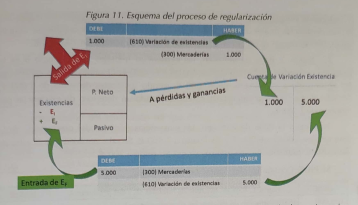
\includegraphics[width=\textwidth]{figura5.png}
\end{figure}

\section*{Regularización de Existencias}

Para situar en el balance el valor de las existencias finales que quedan en el almacén de la empresa, se debe registrar la variación entre las existencias iniciales y finales en la cuenta de pérdidas y ganancias. No hay una única cuenta de "variación de existencias"; el PGC distingue entre las existencias sujetas a transformación (cuentas 71X) y las no sujetas a transformación (cuentas 61X).

\begin{figure}[h]
\centering
\begin{tabular}{|p{4cm}|p{4cm}|p{4cm}|}
\hline
\textbf{Existencias no sujetas a transformación} & $\rightarrow$ & \textbf{Cuenta de variación de existencias 61X} \\
\hline
\textbf{Existencias sujetas a transformación} & $\rightarrow$ & \textbf{Cuenta variación de existencias 71X} \\
\hline
\end{tabular}
\caption{Esquema de regularización de existencias}
\end{figure}

Valoradas las existencias finales, se procede a su contabilización según la NV 10.2, y luego se realiza un test de deterioro si el valor contable es superior al valor de mercado.

\section*{Ejemplo 7}

La empresa DELTA S.A. presenta la siguiente información relativa a sus existencias:

1. Las existencias iniciales del producto A de la empresa ascienden a 100,000 €. Las existencias finales de mercancías, según información extra contable, se valoran en 80,000 €, siendo el valor de mercado a 31 de diciembre de 104,000 €.

2. Según la fecha de almacén, las existencias iniciales del producto B de la empresa son 132,000 € y las finales de 87,000 €. El valor de las existencias finales a 31-12 será de 90,000 €, siendo sus costes de venta de 3,000 €.

3. Según la fecha de almacén, las existencias iniciales del producto C de la empresa son 6,000 € y las finales de 7,500 €. Se sabe también que el valor de mercado de una partida de oficina anterior a 200 €.

\section*{Contabilizar las operaciones anteriores}

\begin{table}[h]
\centering
\begin{tabular}{|c|l|c|}
\hline
\textbf{DEBE} & \textbf{Punto 1. Baja de existencias iniciales (E\textsubscript{i}) del producto A} & \textbf{HABER} \\
\hline
100.000 & (610) Variación de existencias de mercaderías & \\
 & \hspace{2cm} (300) Mercaderías & 100.000 \\
\hline
\textbf{DEBE} & \textbf{Punto 1. Alta de existencias finales (E\textsubscript{f}) del producto A} & \textbf{HABER} \\
\hline
80.000 & (300) Mercaderías & \\
& \hspace{2cm}(610) Variación de existencias de mercaderías & 80.000 \\
\hline
\end{tabular}
\caption{Contabilización de las operaciones del producto A}
\end{table}

Sabiendo que el valor de mercado a 31/12 es superior al valor contable de las mercaderías, no hay deterioro.

\begin{table}[H]
\centering
\begin{tabular}{|c|l|c|}
\hline
\textbf{DEBE} & \textbf{Punto 2. Baja de existencias iniciales (E\textsubscript{i}) del producto B} & \textbf{HABER} \\
\hline
132.000 & (610) Variación de existencias de mercaderías & \\
 & \hspace{2cm} (300) Mercaderías & 132.000 \\
\hline
\end{tabular}
\caption{Baja de existencias iniciales del producto B}
\end{table}

\begin{table}[H]
\centering
\begin{tabular}{|c|l|c|}
\hline
\textbf{DEBE} & \textbf{Punto 2. Alta de existencias finales (E\textsubscript{f}) del producto B} & \textbf{HABER} \\
\hline
87.000 & (300) Mercaderías & \\
 & \hspace{2cm} (610) Variación de existencias de mercaderías & 87.000 \\
\hline
\end{tabular}
\caption{Alta de existencias finales del producto B}
\end{table}

%-------------------------

Para valorar la posibilidad de la existencia de deterioro:

El valor de mercado a 31/12 es de 90.000 €, y los costes de venta 3.000 €, el valor realizable asciende a: 90.000-3.000 = 87.000 €, este importe es igual al valor contable (según la ficha de almacén) de nuestras existencias, luego no hay deterioro, pero tendremos igualmente que revertir el deterioro que teníamos contabilizado del año anterior, es decir:

\begin{table}[H]
\centering
\begin{tabular}{|c|l|c|}
\hline
\textbf{DEBE} & \textbf{Punto 2. Reversión del deterioro del ejercicio anterior} & \textbf{HABER} \\
\hline
2.250 & (390) Deterioro de valor de existencias & \\
 & (7931) Reversión del deterioro de mercaderías & 2.250 \\
\hline
\end{tabular}
\end{table}

\begin{table}[H]
\centering
\begin{tabular}{|c|l|c|}
\hline
\textbf{DEBE} & \textbf{Punto 3. Baja de existencias iniciales (E\textsubscript{i}) del producto C} & \textbf{HABER} \\
\hline
6.000 & (610) Variación de existencias de mercaderías & \\
 & (300) Mercaderías & 6.000 \\
\hline
\textbf{DEBE} & \textbf{Punto 3. Alta de existencias finales (E\textsubscript{f}) del producto C} & \textbf{HABER} \\
\hline
7.500 & (300) Mercaderías & \\
 & (610) Variación de existencias de mercaderías & 7.500 \\
\hline
\end{tabular}
\end{table}

La información del enunciado no nos indica que existan existencias iniciales, luego sólo tendremos que dar de alta las existencias finales.

\begin{table}[H]
\centering
\begin{tabular}{|c|l|c|}
\hline
\textbf{DEBE} & \textbf{Punto 3.2 Alta de existencias finales (E\textsubscript{f}) del material de oficina} & \textbf{HABER} \\
\hline
200 & (328) Material de oficina & \\
 & (612) Variación de existencias de otros aprovisionamientos & 200 \\
\hline
\end{tabular}
\end{table}

\subsection{Impuesto sobre el Valor Añadido (IVA)}

El Impuesto sobre el Valor Añadido (IVA) es un tributo de naturaleza indirecta que recae sobre el consumo y grava, en la forma y condiciones previstas en la ley y reglamento, las entregas de bienes y prestaciones de servicios efectuadas por empresarios y profesionales.

Los impuestos directos gravan el patrimonio, los ingresos o cualquier otra manifestación directa de la riqueza de una persona física o jurídica: impuesto sobre la renta de las personas físicas (IRPF), impuesto sobre sociedades, impuesto sobre bienes inmuebles (IBI), etc.

Los impuestos indirectos, en cambio, gravan la manifestación indirecta de las riquezas de las personas. Por lo tanto, se aplican sobre el consumo y las transmisiones de bienes o derechos: Impuesto sobre el Valor Añadido (IVA), impuesto sobre transmisiones patrimoniales y actos jurídicos documentados.

La base imponible del IVA es la cantidad sobre la que debe aplicarse el tipo impositivo. Estará constituida por el importe total de la contraprestación de las operaciones sujetas al mismo procedente del destinatario o de terceras personas.

El sistema de cálculo se basa en la aplicación de un tipo de gravamen sobre la base imponible, tanto a las salidas (ventas de bienes y servicios), como a las entradas (compras de bienes y servicios), de tal forma que la liquidación del impuesto tendrá lugar por la diferencia entre el IVA repercutido y el IVA soportado. Si esta diferencia es positiva tendremos un IVA a ingresar, en caso contrario, el IVA será a compensar o a devolver. Actualmente hay tres tipos de IVA: general (21\%), reducido (10\%) y super-reducido (4\%).

Todos los operadores mercantiles censados como sujetos pasivos del IVA están obligados a presentar declaraciones trimestrales o mensuales, dependiendo de su volumen de negocio, con independencia de que hayan efectuado operaciones durante el período. Estas declaraciones deben presentarse durante los primeros veinte días naturales del mes siguiente al período de liquidación.

El IVA es un impuesto neutro para la empresa, ya que lo soporta el consumidor final. La empresa actúa como recaudadora para la Hacienda Pública. La contabilización del IVA se realiza de la siguiente manera:

\subsection*{Por la adquisición de bienes y servicios}
\begin{table}[H]
\centering
\begin{tabular}{|c|c|c|}
\hline
\textbf{DEBE} & & \textbf{HABER} \\
\hline
& (600) Compra de mercaderías & \\
\hline
& (472) Hacienda Pública, IVA Soportado & \\ 
\hline
& a (57X) Tesorería & \\
\hline
& a (400) Proveedores & \\
\hline
\end{tabular}
\caption{Registro de adquisición de bienes y servicios}
\end{table}

\subsection*{Por la venta de mercaderías}
\begin{table}[H]
\centering
\begin{tabular}{|c|c|c|}
\hline
\textbf{DEBE} & & \textbf{HABER} \\
\hline
& 57X) Tesorería & \\
\hline
& a (700) Venta de mercaderías & \\
\hline
& (430) Clientes & \\
\hline
& a (477) Hacienda Pública, IVA Repercutido & \\
\hline
\end{tabular}
\caption{Registro de venta de mercaderías}
\end{table}

\subsection{Anticipos a proveedores}

Los anticipos a proveedores son entregas que la empresa realiza en efectivo y se reflejan en el activo corriente del balance bajo el epígrafe ``Existencias''. Esta cuenta, (407) ``Anticipos a proveedores'', muestra que el bien tiene una naturaleza económica y no financiera, condicionando su relación con el IVA.

\subsubsection*{Existencias: Compras y Ventas}
Una cuestión relativa a los anticipos es si se devenga el hecho imponible del IVA. Aunque no se ha producido una entrega de bienes o servicios, el legislador considera que el adelanto implica la intención de entregar dichos bienes o servicios. Por lo tanto, es obligatorio devengar el IVA soportado para el comprador y el repercutido para el vendedor (artículo 75.dos LIVA).


\section*{Ejemplo 8}
Determinada empresa realiza un anticipo para una futura compra de 100 €. Se pide, reflejo contable del mismo teniendo en cuenta el devengo del IVA (21\%). Posteriormente, un mes después se produce la compra de las mercaderías por valor de 500 € (IVA 21\%).

\subsection*{Primera anotación contable:}
\begin{table}[H]
\centering
\begin{tabular}{|c|c|c|}
\hline
\textbf{DEBE} & & \textbf{HABER} \\
\hline
100 & (407) Anticipos a Proveedores & \\
\hline
21 & (472) Hacienda Pública, IVA Soportado & \\ 
\hline
& a (57X) Tesorería & 121 \\
\hline
\end{tabular}
\caption{Anticipo de 100 €}
\end{table}

Cuando se produce la compra por 500 € y se compensa el anticipo. Obsérvese que en el registro contable del IVA sólo se contabiliza por la diferencia entre la compra de 500 € y el IVA del anticipo ya contabilizado previamente.



\subsection*{Segunda anotación contable:}
\begin{table}[H]
\centering
\begin{tabular}{|c|c|c|}
\hline
\textbf{DEBE} & & \textbf{HABER} \\
\hline
500 & (600) Compra de mercaderías & \\
\hline
84 & (472) Hacienda Pública, IVA Soportado [21\% s/ 500-100] & \\ 
\hline
& a (407) Anticipos a Proveedores & 100 \\
\hline
& a (57X) Tesorería & 484 \\
\hline
\end{tabular}
\caption{Compra de mercaderías por 500 €}
\end{table}


\subsection{Anticipos de clientes}

De la misma forma que pueden existir un anticipo a proveedores, es posible que se registre la existencia de anticipos de clientes. Estos se definen como entregas de clientes, normalmente en efectivo, en concepto de «a cuenta» de suministros futuros. La cuenta figurará en el pasivo corriente del balance (438) «Anticipos de clientes». En relación con el impuesto del valor añadido, al igual que sucede con los anticipos a proveedores, en este caso, cuando se produce el anticipo de clientes se produce el devengo del «IVA repercutido».

\textbf{Ejemplo 9.-} Determinada empresa recibe un anticipo de un cliente para una futura venta de 100 €. Se pide, reflejo contable del mismo teniendo en cuenta el futuro devengo de impuesto del valor añadido (IVA 21\%). Posteriormente, un mes después se produce la venta de las mercaderías por valor de 500 € (IVA 21\%).

\begin{center}
\textbf{Por el reflejo contable del anticipo}
\begin{tabular}{|p{5cm}|p{5cm}|p{5cm}|}
\hline
\textbf{DEBE} & & \textbf{HABER} \\
\hline
121 & (57X) Tesorería & \\
\hline
 & (477) Hacienda Pública, IVA repercutido & 21\\
 \hline
 &  (438) Anticipos de Clientes & 100 \\
\hline
\end{tabular}
\end{center}

\begin{center}
\textbf{Cuando se produce la venta por 500 € y se compensa el anticipo:}
\begin{tabular}{|p{5cm}|p{5cm}|p{5cm}|}
\hline
\textbf{DEBE} & & \textbf{HABER} \\
\hline
100 & (438) Anticipos de Clientes & \\
\hline
448 & (57X) Tesorería & \\
\hline
 & a (700) Venta de mercaderías & 500\\
 \hline
 &  a (477) Hacienda Pública, IVA repercutido [21\% s/ 500-100] & 48\\
\hline
\end{tabular}
\end{center}

\subsection{Ejemplo 10}

En el balance de situación de la empresa PROME, S.A. a 01-01-X2 aparecen, entre otras partidas:

\begin{itemize}
    \item (300) Mercaderías: 70.000 €
    \item (390) Deterioro de valor de las mercaderías: 2.000 €
\end{itemize}

Durante el último trimestre del ejercicio X2 la empresa ha realizado las siguientes operaciones con sus mercaderías (IVA de las operaciones 21\%):

\begin{itemize}
    \item Compra a crédito 10.000 unidades del producto a 8 €/unidad, con un descuento comercial del 10\%, y un descuento en factura por volumen de pedido de 3.600 €. El transporte asciende a 600 € quedando pendiente de pago.
    \item Entrega un anticipo a un proveedor a cuenta de suministros futuros por importe de 5.000 €.
    \item Vende mercaderías al contado por valor de 100.000 € a un cliente que nos había entregado un anticipo de 10.000 € en el año X1, aplicándole un descuento en factura del 10\% del total de la venta.
    \item Por defectos de calidad, PROME, S.A. devuelve una partida de mercaderías por importe de 8.000 €. Como ya estaba pagado, las empresas pactan considerarlo como un anticipo a cuenta de futuras compras.
    \item Un proveedor nos concede un descuento gracias al volumen de compras que le ha hecho la empresa por valor de 3.000 €. Dicho importe se considera como una menor deuda con ese proveedor.
    \item A 31-12-X2 la empresa tiene unas existencias finales valoradas en 50.000 €, pero en un recuento físico de las mismas, se ha detectado una partida valorada en 1.000 € que se considera inservible para la venta. El precio de venta de dichas mercaderías es de 51.000 € y los costes de comercialización se calculan en 3.000 €.
\end{itemize}

\textbf{SE PIDE:} Teniendo en cuenta la información anterior, contabilizar:
\begin{enumerate}
    \item Compra de las mercancías.
    \item Venta de las mercancías.
    \item Devolución de las mercancías.
    \item Descuento por volumen.
    \item Contabilización del deterioro reversible e irreversible de mercancías a 31/12/X2.
\end{enumerate}

\textbf{SOLUCIÓN.}

En este ejercicio no es necesario trabajar con la ficha de almacén, puesto que nos dan la información de las existencias finales a 31/12/X2. Ahora bien, para resolver el apartado e) debemos tener en cuenta la información inicial, donde nos indican que la empresa tenía contabilizado un deterioro de mercancías del año X1 por importe de 2.000 €.

\subsection*{ Compra de las mercaderías}

Debemos calcular el precio de adquisición:
\begin{align*}
    \text{PA} &= \text{Factura} - \text{descuentos en factura} + \text{gastos necesarios} \\
    \text{PA} &= \left[ (10.000 \times 8) \times 90\% (3) \right] - 3.600(4) + 600 = 69.000 \, \text{€}
\end{align*}

Como la compra es a crédito, se contabilizará una deuda con los proveedores (con su IVA correspondiente) por importe de:
\begin{align*}
    \left[ 10.000 \times 8 \times 90\% \right] - 3.600 = 68.400 \, \text{€} + 21\% \times 68.400 = 82.764 \, \text{€}
\end{align*}

Los gastos de transporte también quedan pendientes de pago. Como se ha visto en ejercicios anteriores, se recoge en la cuenta (410) Acreedores por prestación de servicios, junto con el IVA correspondiente a este servicio, es decir:
\begin{align*}
    600 + 21\% \times 600 = 726 \, \text{€}
\end{align*}

\begin{table}[H]
\centering
\begin{tabular}{|c|c|c|}
\hline
\textbf{DEBE} & \textbf{Compra de las mercancías} & \textbf{HABER} \\
\hline
69.000 & (600) Compra de mercancías & \\
14.490 & (472) H.P. IVA Soportado (5)& \\
& (400) Proveedores & 82.764 \\
& (410) Acreedores por prestación de servicios & 726 \\
\hline
\end{tabular}
\end{table}

\textit{Explicación:} 
\begin{itemize}
    \item La cuenta (600) Compra de mercancías se carga con el precio de adquisición calculado (69.000 €).
    \item La cuenta (472) H.P. IVA Soportado se carga con el IVA correspondiente a la compra (21\% de 69.000 € = 14.490 €).
    \item La cuenta (400) Proveedores se abona con el total de la deuda (68.400 € + 21\% de 68.400 € = 82.764 €).
    \item La cuenta (410) Acreedores por prestación de servicios se abona con el total del transporte pendiente de pago (600 € + 21\% de 600 € = 726 €).
\end{itemize}

\subsection*{Entrega del anticipo}

\begin{table}[H]
\centering
\begin{tabular}{|c|c|c|}
\hline
\textbf{DEBE} & & \textbf{HABER} \\
\hline
5.000 & (407) Anticipo a proveedores & \\
1.050 & (472) H.P. IVA Soportado & \\
 & & (572) Bancos c/c 6.050 \\
\hline
\end{tabular}
\caption{Entrega del anticipo}
\end{table}

\textit{Explicación:} 
\begin{itemize}
    \item La cuenta (407) Anticipo a proveedores se carga con el importe del anticipo (5.000 €).
    \item La cuenta (472) H.P. IVA Soportado se carga con el IVA correspondiente al anticipo (21\% de 5.000 € = 1.050 €).
    \item La cuenta (572) Bancos c/c se abona con el total del anticipo más el IVA (5.000 € + 1.050 € = 6.050 €).
\end{itemize}

\subsection*{Venta de las mercancías}

\begin{table}[H]
\centering
\begin{tabular}{|c|c|c|}
\hline
\textbf{DEBE} & & \textbf{HABER} \\
\hline
10.000 & (438) Anticipo de clientes & \\
96.800 & (570) Caja, euros & \\
 & & (700) Vta. mercaderías 90.000 \\
 & & (477) H. P. IVA repercutido 16.800 \\
\hline
\end{tabular}
\caption{Venta de las mercancías}
\end{table}

\textit{Explicación:} 
\begin{itemize}
    \item La cuenta (438) Anticipo de clientes se carga con el importe del anticipo recibido (10.000 €).
    \item La cuenta (570) Caja, euros se carga con el importe recibido al contado (100.000 € - 10.000 € de anticipo = 90.000 €).
    \item La cuenta (700) Venta de mercaderías se abona con el valor de la venta (100.000 € - 10\% de 100.000 € = 90.000 €).
    \item La cuenta (477) H.P. IVA repercutido se abona con el IVA correspondiente a la venta (21\% de 90.000 € = 16.800 €).
\end{itemize}

\subsection*{Devolución de las mercaderías}

\begin{itemize}
    \item Si hay que contabilizar exclusivamente la devolución de una partida de mercancías por importe de 8.000, se realizaría teniendo en cuenta que se le devuelve el IVA correspondiente.
\end{itemize}

\subsection*{Devolución de mercancías}

\begin{table}[H]
\centering
\begin{tabular}{|c|c|c|}
\hline
\textbf{DEBE} & & \textbf{HABER} \\
\hline
9.680 & (572) Bancos c/c & \\
 & (608) Devolución de compras y operaciones similares & 8.000 \\
 & (472) H.P. IVA Soportado & 1.680 \\
\hline
\end{tabular}
\caption{Devolución de mercancías}
\end{table}

\textit{Explicación:} 
\begin{itemize}
    \item La cuenta (572) Bancos c/c se carga con el importe total de la devolución (8.000 € + 21\% de 8.000 € = 9.680 €).
    \item La cuenta (608) Devolución de compras y operaciones similares se abona con el importe de la devolución (8.000 €).
    \item La cuenta (472) H.P. IVA Soportado se abona con el IVA correspondiente a la devolución (21\% de 8.000 € = 1.680 €).
\end{itemize}

\subsection*{Entrega de un anticipo a un proveedor}

\begin{table}[H]
\centering
\begin{tabular}{|c|c|c|}
\hline
\textbf{DEBE} & & \textbf{HABER} \\
\hline
8.000 & (407) Anticipos a proveedores & \\
1.680 & (472) H.P. IVA Soportado & \\
 & & (572) Bancos c/c 9.680 \\
\hline
\end{tabular}
\caption{Entrega de un anticipo a un proveedor}
\end{table}

\textit{Explicación:} 
\begin{itemize}
    \item La cuenta (407) Anticipos a proveedores se carga con el importe del anticipo (8.000 €).
    \item La cuenta (472) H.P. IVA Soportado se carga con el IVA correspondiente al anticipo (21\% de 8.000 € = 1.680 €).
    \item La cuenta (572) Bancos c/c se abona con el total del anticipo más el IVA (8.000 € + 1.680 € = 9.680 €).
\end{itemize}

\subsection*{Descuento por volumen}

\begin{table}[H]
\centering
\begin{tabular}{|c|c|c|}
\hline
\textbf{DEBE} & & \textbf{HABER} \\
\hline
3.630 & (400) Proveedores & \\
 & (609) Rappels por compras & 3.000 \\
 & (472) H.P. IVA Soportado & 630 \\
\hline
\end{tabular}
\caption{Descuento por volumen}
\end{table}

\textit{Explicación:} 
\begin{itemize}
    \item La cuenta (400) Proveedores se carga con el importe total del descuento más el IVA (3.000 € + 21\% de 3.000 € = 3.630 €).
    \item La cuenta (609) Rappels por compras se abona con el importe del descuento (3.000 €).
    \item La cuenta (472) H.P. IVA Soportado se abona con el IVA correspondiente al descuento (21\% de 3.000 € = 630 €).
\end{itemize}

\subsection*{Contabilización del deterioro reversible e irreversible de las mercancías}
A 31/12/X2, la empresa tiene existencias finales valoradas en 50.000 €. En un recuento físico de las mismas, se detectó una partida valorada en 1.000 € inservible para la venta. La NRV 10.2 indica que cuando una depreciación de existencias es irreversible, debe reflejarse en la valoración de las existencias finales, mostrando la pérdida de forma correspondiente.

\section*{Contabilización del deterioro de mercaderías a 31/12/X2}

El valor de las existencias finales es de 50.000 €, pero al considerar las existencias depreciadas de 1.000 €, el valor contable es de 49.000 €. Se plantean dos cuestiones:

1. ¿Existe deterioro de mercaderías del año anterior? Sí, hay un deterioro de 2.000 €, que se debe revertir.
2. ¿Existe deterioro de mercaderías para este año? El test de deterioro indica que el valor neto realizable es 48.000 €, inferior al valor contable de 49.000 €, lo que implica un deterioro de 1.000 €.

\begin{table}[H]
\centering
\begin{tabular}{|c|p{4cm}|p{3cm}|}
\hline
\textbf{DEBE} & Contabilización del deterioro reversible e irreversible de mercaderías a 31/12/X2 & \textbf{HABER} \\
\hline
2.000 & (390) Deterioro de valor de las mercaderías & \\
 & & (793) Reversión del deterioro de existencias 2.000 \\
1.000 & (693) Pérdidas por deterioro de existencias & \\
 & & (390) Deterioro de valor de las mercaderías 1.000 \\
\hline
\end{tabular}
\end{table}

\textit{Explicación:} 
\begin{itemize}
    \item La cuenta (390) Deterioro de valor de las mercaderías se carga con el importe del deterioro del año anterior (2.000 €) y se abona con el importe de la reversión del deterioro (2.000 €).
    \item La cuenta (693) Pérdidas por deterioro de existencias se carga con el importe del deterioro del año actual (1.000 €).
    \item La cuenta (390) Deterioro de valor de las mercaderías se abona con el importe del deterioro del año actual (1.000 €).
\end{itemize}


\subsection{Ejemplo 11}

La empresa MAGRA S.A. ha realizado durante los últimos meses las siguientes operaciones relacionadas con la compra de mercaderías:

1. El 2 de noviembre se compran mercaderías por 2.600 €, con un descuento de 100 € y un gasto de transporte de 300 €, pagado mediante transferencia bancaria. (IVA 21%)
2. El 2 de noviembre se compran mercaderías a crédito por 2.600 €, con un descuento de 100 € y un gasto de transporte de 300 €, pagado mediante transferencia bancaria. (IVA 21%)
3. El 2 de noviembre se compran mercaderías a crédito por 2.600 €, con un descuento de 100 € y un gasto de transporte de 300 € a crédito. (IVA 21%)
4. Compra mercaderías por 1.000 €, paga 500 € mediante cheque. Descuento por pronto pago del 5% dentro de factura y un gasto de transporte de 75 €, pendiente de pago. (IVA 21%)

\subsection*{Punto 1}
\begin{table}[H]
\centering
\begin{tabular}{|c|c|c|}
\hline
\textbf{DEBE} & \textbf{Descripción} & \textbf{HABER} \\
\hline
2.800 & (600) Compra de mercaderías &  \\
588 & (472) H.P. IVA Soportado &  \\
 & & (572) Bancos c/c 3.388 \\
\hline
\end{tabular}
\end{table}

\textit{Cálculo:}
\begin{itemize}
    \item \textbf{(600) Compra de mercaderías:} 2.600 € - 100 € (descuento) + 300 € (transporte) = 2.800 €
    \item \textbf{(472) H.P. IVA Soportado:} 21\% de 2.800 € = 588 €
    \item \textbf{(572) Bancos c/c:} 2.800 € + 588 € = 3.388 €
\end{itemize}

\subsection*{Punto 2}
\begin{table}[H]
\centering
\begin{tabular}{|c|c|c|}
\hline
\textbf{DEBE} & \textbf{Descripción} & \textbf{HABER} \\
\hline
2.800 & (600) Compra de mercaderías &  \\
588 & (472) H.P. IVA Soportado &  \\
 & & (400) Proveedores 3.025 \\
 & & (572) Bancos c/c 363 \\
\hline
\end{tabular}
\end{table}

\textit{Cálculo:}
\begin{itemize}
    \item \textbf{(600) Compra de mercaderías:} 2.600 € - 100 € (descuento) + 300 € (transporte) = 2.800 €
    \item \textbf{(472) H.P. IVA Soportado:} 21\% de 2.800 € = 588 €
    \item \textbf{(400) Proveedores:} 2.600 € - 100 € (descuento) = 2.500 € + 21\% de 2.500 € = 3.025 €
    \item \textbf{(572) Bancos c/c:} 300 € (transporte) + 21\% de 300 € = 363 €
\end{itemize}

\subsection*{Punto 3}
\begin{table}[H]
\centering
\begin{tabular}{|c|c|c|}
\hline
\textbf{DEBE} & \textbf{Descripción} & \textbf{HABER} \\
\hline
2.800 & (600) Compra de mercaderías &  \\
588 & (472) H.P. IVA Soportado &  \\
 & & (400) Proveedores 3.388 \\
\hline
\end{tabular}
\end{table}

\textit{Cálculo:}
\begin{itemize}
    \item \textbf{(600) Compra de mercaderías:} 2.600 € - 100 € (descuento) + 300 € (transporte) = 2.800 €
    \item \textbf{(472) H.P. IVA Soportado:} 21\% de 2.800 € = 588 €
    \item \textbf{(400) Proveedores:} 2.800 € + 588 € = 3.388 €
\end{itemize}

\subsection*{Punto 4}
\begin{table}[H]
\centering
\begin{tabular}{|c|c|c|}
\hline
\textbf{DEBE} & \textbf{Descripción} & \textbf{HABER} \\
\hline
1.000 & (600) Compra de mercaderías &  \\
210 & (472) H.P. IVA Soportado &  \\
 & & (572) Bancos c/c 500 \\
 & & (410) Acreedores por prestación de servicios 75 \\
\hline
\end{tabular}
\end{table}

\textit{Cálculo:}
\begin{itemize}
    \item \textbf{(600) Compra de mercaderías:} 1.000 € - 5\% de 1.000 € (descuento) + 75 € (transporte) = 1.025 €
    \item \textbf{(472) H.P. IVA Soportado:} 21\% de 1.025 € = 215,25 €
    \item \textbf{(572) Bancos c/c:} 500 €
    \item \textbf{(410) Acreedores por prestación de servicios:} 75 €
\end{itemize}

\section*{Contabilización de Operaciones de Compra}

\subsection*{Compra a Crédito}
En este caso, tanto la adquisición de las mercaderías como el transporte se realizan a crédito. Las cuentas utilizadas para reflejar esta deuda comercial son:

\begin{table}[H]
\centering
\begin{tabular}{|c|c|c|}
\hline
\textbf{DEBE} & \textbf{Descripción} & \textbf{HABER} \\
\hline
2.800 & (600) Compra de mercaderías & \\
588 & (472) H.P. IVA Soportado & \\
 & (400) Proveedores & 3.025 \\
 & (410) Acreedores por prestación de servicios & 363 \\
\hline
\end{tabular}
\caption{Registro de compra a crédito}
\end{table}

\textit{Cálculo:}
\begin{itemize}
    \item \textbf{(600) Compra de mercaderías:} 2.600 € - 100 € (descuento) + 300 € (transporte) = 2.800 €
    \item \textbf{(472) H.P. IVA Soportado:} 21\% de 2.800 € = 588 €
    \item \textbf{(400) Proveedores:} 2.600 € - 100 € (descuento) = 2.500 € + 21\% de 2.500 € = 3.025 €
    \item \textbf{(410) Acreedores por prestación de servicios:} 300 € (transporte) + 21\% de 300 € = 363 €
\end{itemize}

\subsection*{Descuento por Pronto Pago Incluido en Factura}
La operación refleja un descuento financiero en factura descontado del importe de adquisición y se incluye el gasto de transporte.

\begin{table}[H]
\centering
\begin{tabular}{|c|c|c|}
\hline
\textbf{DEBE} & \textbf{Descripción} & \textbf{HABER} \\
\hline
1.025 & (600) Compra de mercaderías & \\
215,25 & (472) H.P. IVA Soportado & \\
 & (572) Bancos c/c & 500 \\
 & (400) Proveedores & 649,75 \\
 & (410) Acreedores por prestación de servicios & 90,75 \\
\hline
\end{tabular}
\caption{Descuento por pronto pago incluido en factura}
\end{table}

\textit{Cálculo:}
\begin{itemize}
    \item \textbf{Descuento (en factura):} 5\% de 1.000 € = 50 €
    \item \textbf{Transportes:} 75 €
    \item \textbf{Precio de adquisición:} 1.000 € - 50 € + 75 € = 1.025 €
    \item \textbf{(472) H.P. IVA Soportado:} 21\% de 1.025 € = 215,25 €
    \item \textbf{(572) Bancos c/c:} 500 €
    \item \textbf{(400) Proveedores:} 1.025 € - 500 € = 525 € + 21\% de 525 € = 649,75 €
    \item \textbf{(410) Acreedores por prestación de servicios:} 75 € + 21\% de 75 € = 90,75 €
\end{itemize}

\begin{tcolorbox}[colback=blue!5!white, colframe=blue!75!black, title=Plus]
\subsection*{Ejemplo 12 esta en el libro.}
\end{tcolorbox}

%---------------------------------

\subsection{Envases y embalajes}

La valoración de las existencias incluye la contabilización de los envases y embalajes adquiridos o vendidos con mercaderías. Las cuentas involucradas son:

\begin{itemize}
    \item (406) \textbf{Envases y embalajes a devolver a proveedores}: Registra el importe de envases y embalajes cargados en factura por proveedores con derecho a devolución. Figura en el pasivo corriente del balance.
    \item (437) \textbf{Envases y embalajes a devolver por clientes}: Registra el importe de envases y embalajes cargados en factura a clientes con derecho a devolución. Figura en el activo corriente del balance.
\end{itemize}

Las anotaciones contables derivadas de envases y embalajes son:

\section*{Proveedores}

\subsection*{Envases y embalajes a devolver a proveedores}

\begin{table}[H]
\centering
\begin{tabular}{|p{4cm}|p{4cm}|p{4cm}|}
\hline
\textbf{DEBE} & \textbf{Descripción} & \textbf{HABER} \\
\hline
& (600) Compras de mercaderías & \\
& (406) Envases y embalajes a devolver a proveedores & \\
& (472) H.P. IVA soportado & \\
&  (400) Proveedores & \\
\hline
\end{tabular}
\caption{Contabilización de envases y embalajes a devolver a proveedores}
\end{table}

\subsection*{Devolución de envases y embalajes a proveedores}

\begin{table}[H]
\centering
\begin{tabular}{|p{4cm}|p{4cm}|p{4cm}|}
\hline
\textbf{DEBE} & \textbf{Descripción} & \textbf{HABER} \\
\hline
& (400) Proveedores & \\
&  (406) Envases y embalajes a devolver a proveedores & \\
&  (472) H.P. IVA soportado & \\
\hline
\end{tabular}
\caption{Contabilización de la devolución de envases y embalajes a proveedores}
\end{table}

\subsection*{Adquisición de envases y embalajes}

Si la empresa adquiere en propiedad los envases y embalajes, pierde el derecho a devolución y se registra como una compra de otros aprovisionamientos:

\begin{table}[H]
\centering
\begin{tabular}{|p{4cm}|p{4cm}|p{4cm}|}
\hline
\textbf{DEBE} & \textbf{Descripción} & \textbf{HABER} \\
\hline
& (602) Compras de otros aprovisionamientos & \\
&  (406) Envases y embalajes a devolver a proveedores & \\
\hline
\end{tabular}
\caption{Contabilización cuando la empresa se queda con los envases y embalajes}
\end{table}

\section*{Clientes}

Para el caso de los envases y embalajes a devolver por el cliente, las anotaciones contables quedarían de la siguiente forma:

\begin{table}[H]
\centering
\begin{tabular}{|p{4cm}|p{4cm}|p{4cm}|}
\hline
\textbf{DEBE} & \textbf{Contabilización de envases y embalajes a devolver por clientes, con derecho a devolución} & \textbf{HABER} \\
\hline
& \textcolor{blue}{(430) Clientes} & \\
& \textcolor{red}{(700) Ventas de mercaderías} & \\
& \textcolor{green}{(437) Envases y embalajes a devolver por clientes} & \\
& \textcolor{purple}{(477) H.P. IVA repercutido} & \\
\hline
\end{tabular}
\caption{Contabilización de envases y embalajes a devolver por clientes}
\end{table}

\begin{table}[H]
\centering
\begin{tabular}{|p{4cm}|p{4cm}|p{4cm}|}
\hline
\textbf{DEBE} & \textbf{Contabilización de la devolución de los envases y embalajes a devolver por clientes} & \textbf{HABER} \\
\hline
& \textcolor{green}{(437) Envases y embalajes a devolver por clientes} & \\
& \textcolor{purple}{(477) H.P. IVA repercutido} & \\
& \textcolor{blue}{(430) Clientes} & \\
\hline
\end{tabular}
\caption{Devolución de envases y embalajes a clientes}
\end{table}

\begin{table}[H]
\centering
\begin{tabular}{|p{4cm}|p{4cm}|p{4cm}|}
\hline
\textbf{DEBE} & \textbf{Contabilización cuando el cliente se queda con los envases y embalajes} & \textbf{HABER} \\
\hline
& \textcolor{green}{(437) Envases y embalajes a devolver por clientes} & \\
& \textcolor{orange}{(704) Ventas de embalajes y envases} & \\
\hline
\end{tabular}
\caption{Contabilización de envases y embalajes no devueltos por clientes}
\end{table}

\subsection{Ejemplo 13}

\textbf{Ejemplo 13.-} La empresa AULAGA S.A. dedicada a la comercialización de botellas de aceite al por mayor, realiza las siguientes operaciones el último trimestre:\\

1. El 10/10/2019 adquiere 10.000 litros de aceite a 1,15 €/litro. Los costes de transporte, a cargo de AULAGA ascienden a 700 €. El aceite viene en envases que hay que devolver, cuyo importe es de 1.200 €. AULAGA paga los gastos de transporte y 5.000 euros, dejando el resto a deber.\\

2. El 30/10/2019 devuelve el 90\% de los envases, habiéndose roto el 10\% restante.\\

3. El 20/11/2019 paga otros 5.000 € al proveedor de la compra del 10/10/2019 y el proveedor nos concede un descuento por volumen de 1.000 €.\\

4. El 10/12/2019, la empresa proveedora del aceite, cierra por jubilación del propietario, quedando cancelada toda posible deuda con la misma de manera irrevocable.\\

\textbf{SE PIDE:} Sabiendo que todas las operaciones están sujetas al porcentaje de 21\% de IVA, contabilice las mismas en el libro diario.\\

Al registrar la compra de mercaderías del punto 1, se debe considerar que la cuenta 600. «Compra de mercaderías» incluye el gasto de transporte. Como los envases y embalajes presentan facultad de devolución, tiene que contabilizarse en la cuenta 406. «Envases y embalajes a Devolver a Proveedores». Obsérvese que el IVA de la operación incluye el importe de la compra, el transporte, y los envases y embalajes.\\

\section*{Punto 1}

\begin{table}[H]
\centering
\begin{tabular}{|p{4cm}|p{4cm}|p{4cm}|}
\hline
\textbf{DEBE} & \textbf{Descripción} & \textbf{HABER} \\
\hline
12.200 & (600) Compra de Mercaderías & \\
1.200 & (406) Envases y embalajes a Devolver a Proveedores & \\
2.814 & (472) H.P. IVA Soportado & \\
& & (400) Proveedores \\
& & (572) Banco c/c \\
\hline
\end{tabular}
\caption{Contabilización de la compra de mercaderías}
\end{table}

\textit{Cálculo:}
\begin{itemize}
    \item \textbf{(600) Compra de Mercaderías:} 10.000 litros \(\times\) 1,15 €/litro + 700 € (transporte) = 12.200 €
    \item \textbf{(406) Envases y embalajes a Devolver a Proveedores:} 1.200 €
    \item \textbf{(472) H.P. IVA Soportado:} 21\% de (12.200 € + 1.200 €) = 2.814 €
    \item \textbf{(400) Proveedores:} 12.200 € + 1.200 € + 2.814 € - 5.000 € (pago inicial) = 11.214 €
    \item \textbf{(572) Banco c/c:} 5.000 € (pago inicial) + 700 € (transporte) = 5.700 €
\end{itemize}

\section*{Punto 2}

En este apartado, la empresa debe quedarse con los envases rotos, registrándolos en la cuenta (602) \textit{Compras de Otros Aprovisionamientos}. El resto se devuelve cargando la cuenta de proveedores.

\begin{table}[H]
\centering
\begin{tabular}{|p{4cm}|p{4cm}|p{4cm}|}
\hline
\textbf{DEBE} & \textbf{Descripción} & \textbf{HABER} \\
\hline
1.306,80 & (400) Proveedores & \\
120 & (602) Compras de Otros Aprovisionamientos & \\
& & (406) Envases y embalajes a Devolver a Proveedores \\
& & (472) H.P. IVA Soportado \\
\hline
\end{tabular}
\caption{Devolución de los envases y embalajes}
\end{table}

\textit{Cálculo:}
\begin{itemize}
    \item \textbf{(400) Proveedores:} 90\% de 1.200 € = 1.080 € + 21\% de 1.080 € = 1.306,80 €
    \item \textbf{(602) Compras de Otros Aprovisionamientos:} 10\% de 1.200 € = 120 €
    \item \textbf{(406) Envases y embalajes a Devolver a Proveedores:} 1.200 €
    \item \textbf{(472) H.P. IVA Soportado:} 21\% de 120 € = 25,20 €
\end{itemize}

\section*{Punto 3}

Reflejo contable del apartado 3.

\begin{table}[H]
\centering
\begin{tabular}{|p{4cm}|p{4cm}|p{4cm}|}
\hline
\textbf{DEBE} & \textbf{Descripción} & \textbf{HABER} \\
\hline
6.210 & (400) Proveedores & \\
& & (572) Banco c/c \\
& & (609) Rappels sobre compras \\
& & (472) H.P. IVA Soportado \\
\hline
\end{tabular}
\caption{Pago al proveedor y descuentos por volumen}
\end{table}

\textit{Cálculo:}
\begin{itemize}
    \item \textbf{(400) Proveedores:} 5.000 € (pago) + 1.000 € (descuento) + 21\% de 1.000 € (IVA) = 6.210 €
    \item \textbf{(572) Banco c/c:} 5.000 €
    \item \textbf{(609) Rappels sobre compras:} 1.000 €
    \item \textbf{(472) H.P. IVA Soportado:} 21\% de 1.000 € = 210 €
\end{itemize}

\section*{Punto 4}

En este caso, al extinguirse el pasivo, se considera como un ingreso para la entidad.

\begin{table}[H]
\centering
\begin{tabular}{|p{4cm}|p{4cm}|p{4cm}|}
\hline
\textbf{DEBE} & \textbf{Descripción} & \textbf{HABER} \\
\hline
2.850,20 & (400) Proveedores & \\
& & (778) Ingresos Extraordinarios \\
\hline
\end{tabular}
\caption{Cancelación de la deuda por cierre del proveedor}
\end{table}

\textit{Cálculo:}
\begin{itemize}
    \item \textbf{(400) Proveedores:} 2.850,20 €
    \item \textbf{(778) Ingresos Extraordinarios:} 2.850,20 €
\end{itemize}

\subsection{Coste de las existencias en la prestación de los servicios}

De acuerdo con la NV 10.1.4, los criterios indicados para la valoración de existencias resultarán aplicables para determinar el coste de las existencias de los servicios. En concreto, las existencias incluirán el coste de producción de los servicios en tanto aún no se haya reconocido el ingreso por prestación de servicios.

La propia NV 10.1.4 nos deriva a la NV 14 para completar la valoración del coste de la prestación de servicios. Concretamente, la NV 14.2, establece que para cada obligación a cumplir (entrega de bienes o prestación de servicios) que se hubiera identificado, la empresa determinará al comienzo del contrato si el compromiso asumido se cumplirá a lo largo del tiempo o en un momento determinado.

Tal y como se ha comentado en el epígrafe 2.4.2 del presente capítulo, cuando los ingresos derivados de los compromisos (con carácter general, de prestaciones de servicios) que se cumplen a lo largo del tiempo, éstos se reconocerán en función del grado de avance o progreso hacia el cumplimiento completo de las obligaciones contractuales siempre que la empresa disponga de información fiable para realizar la medición del grado de avance.

En el caso de las obligaciones contractuales que se cumplen en un momento determinado, los ingresos derivados de su ejecución se reconocerán en tal fecha. Hasta que no se produzca esta circunstancia, los costes incurridos en la producción o fabricación del producto (bienes o servicios) se contabilizarán como existencias.

\section*{Ejemplo 14.-} La empresa \textbf{ELECTRONOR} se dedica a la instalación de redes eléctricas para empresas. El 01-01-2019 firma un contrato con la empresa \textbf{EDEVESA} para realizar un proyecto de instalación en una de sus fábricas.

El precio total estipulado en el contrato es de 20.000 euros. Los costes estimados de tales servicios por parte \textbf{ELECTRONOR} son de 10.000 euros que se distribuyen de la siguiente manera:

\begin{itemize}
    \item Año 2019: Mano de obra de personal \dots 6.000 €
    \item Año 2020: Mano de obra del personal \dots 4.000 €
    \item Total \dots 10.000 €
\end{itemize}

El 30-01-2020 se finaliza la instalación y se da el visto bueno por parte de EDEVESA abonando ésta el importe del mismo.

\textbf{SE PIDE:} Determinar el registro contable de la operación anterior en 2019 sabiendo que no se cumplen las condiciones para reconocerlo como ingresos.

\textbf{Solución.} Tal y como se ha comentado en la exposición teórica, un aspecto clave para el reconocimiento de los costes de la prestación de un servicio como un tipo de existencia, es que no se cumplan las condiciones para llevar a cabo su reconocimiento como ingreso, siendo esta condición la que se introduce en el enunciado. Esta situación implica que, desde el punto de vista contable, no es posible llevar a cabo el reconocimiento de un ingreso en el año 2019.

Por tanto, los gastos de mano de obra en los que incurre la empresa en el período 2019, serán considerados como un tipo de existencia. Desde el punto de vista contable, en primer lugar, debemos reconocer el gasto en que incurre la empresa por la mano de obra, aunque esta operación es objeto de estudio en el capítulo 4 del presente manual, procedemos a su contabilización a efectos de explicar su reconocimiento posterior como existencia.

\begin{table}[h!]
\centering
\begin{tabular}{|c|p{4cm}|c|}
\hline
\textbf{DEBE} & \textbf{Contabilización de los gastos de mano de obra en 2019} & \textbf{HABER} \\
\hline
6.000 & (640) Sueldos y salarios & (572) Banco X c/c \\
\hline
\end{tabular}
\end{table}

Al no ser posible contabilizar un ingreso relacionado con este servicio (proyecto) debe considerarse este gasto como un tipo de existencia y, por tanto, determinar su coste, en este caso, 6.000 € y proceder a realizar la variación de existencias. Obsérvese que este proyecto surge en este año, por lo que no tenemos existencias iniciales, y no procede realizar reconocimiento contable de éstas. Las existencias finales ascienden a 6.000 € y este sería el valor de las existencias finales, tal y como se recoge en el siguiente asiento contable.

\begin{table}[h!]
\centering
\begin{tabular}{|c|p{4cm}|c|}
\hline
\textbf{DEBE} & \textbf{Variación de existencias finales en 2019} & \textbf{HABER} \\
\hline
6.000 & (33X) Servicios en curso & (710) Variación de existencias en servicios en curso \\
\hline
\end{tabular}
\end{table}

\begin{figure}[H]
    \centering
    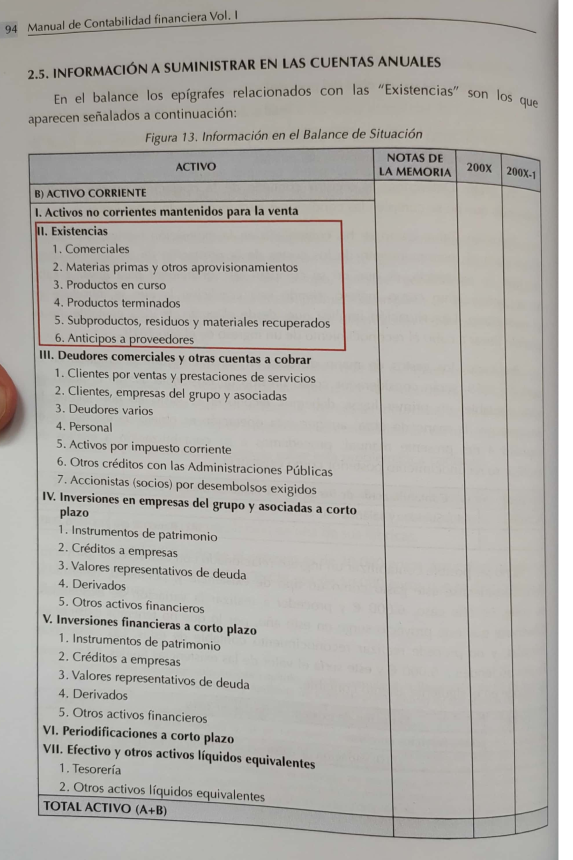
\includegraphics[width=\textwidth]{Cuentas1.png}
\end{figure}

\begin{figure}[H]
    \centering
    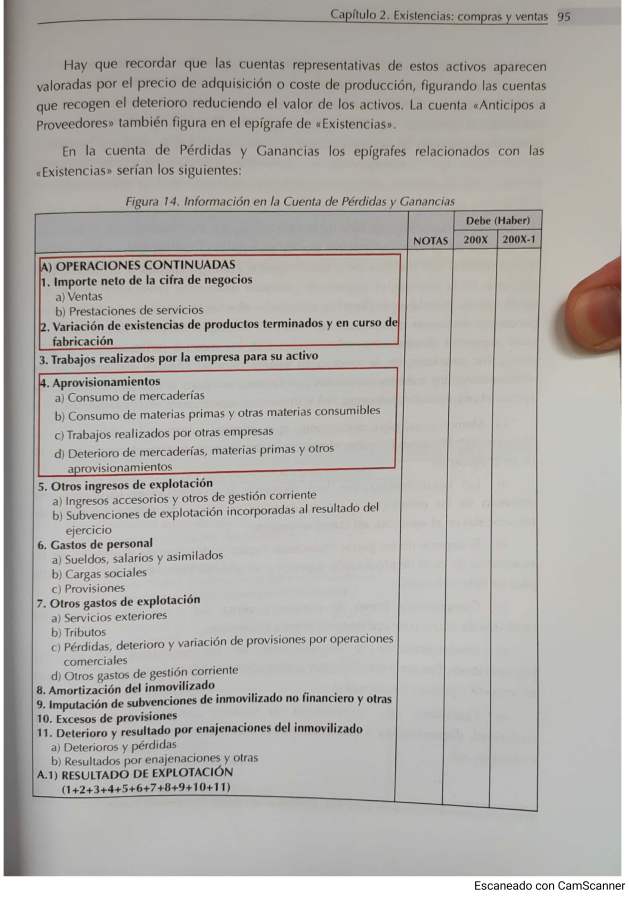
\includegraphics[width=\textwidth]{cuentas2.png}
\end{figure}

La RICAC (2021) permite configurar elementos de la contabilidad, precisando que los ingresos ordinarios son aquellos obtenidos de forma regular y periódica. El importe neto de la cifra de negocios se determina deduciendo varios conceptos, como descuentos y devoluciones. La memoria contable debe incluir información sobre las existencias, como correcciones valorativas, gastos financieros capitalizados, compromisos de compra y venta, limitaciones en la disponibilidad, y otras circunstancias que afecten la titularidad y valoración de las existencias.

\begin{figure}[H]
    \centering
    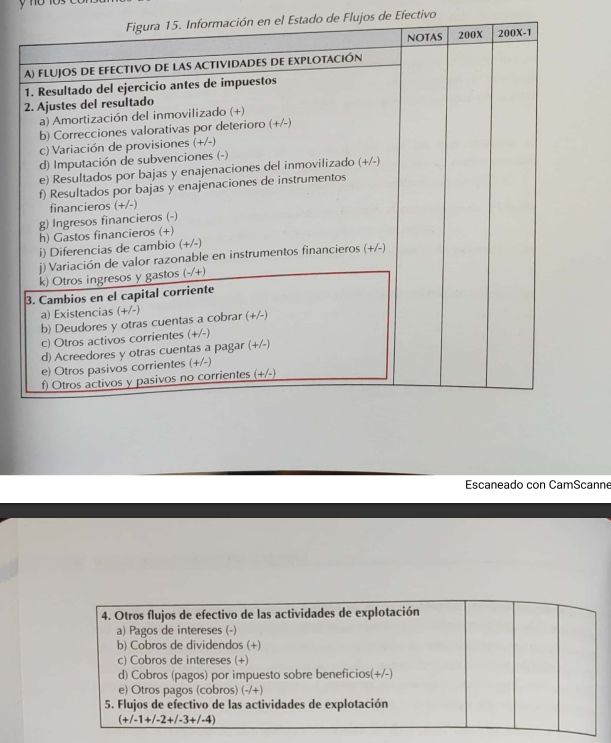
\includegraphics[width=\textwidth]{cuentas3.png}
\end{figure}


De acuerdo con la Nota 13.1 de la Memoria relativa a Ingresos y Gastos, la empresa debe proporcionar información suficiente que permita a los usuarios de las cuentas anuales comprender la naturaleza, importe, calendario e incertidumbre de los ingresos de actividades ordinarias y flujos de efectivo que surgen de contratos con clientes.

Por su parte la Nota 13.5 de la Memoria establece la obligación de informar sobre el desglose de las partidas 4.a) y 4.b) de la cuenta de pérdidas y ganancias “Consumo de mercaderías” y “Consumo de materias primas y otras materias consumibles”, distinguiendo entre compras y variación de existencias. También se diferenciarán las compras nacionales, las adquisiciones intracomunitarias y las importaciones.

Por último, el impacto de las operaciones de existencias en el Estado de Flujos de Efectivo debe reflejarse ajustando la variación de existencias en el apartado de cambios en el capital corriente, para reflejar las compras del período y no los consumos de mercaderías que muestra la cuenta de pérdidas y ganancias.


%---------------------
\begin{tcolorbox}[colback=green!5!white, colframe=blue!75!black, title=Plus]
\subsection*{En el libro de teoría hay otros casos propuestos para realizar.}
\end{tcolorbox}


\end{document}